%
%****************************************************************************************************
%======================= B E G I N   D O C U M E N T   S E T T I N G S ========================
%****************************************************************************************************
%
\documentclass[a4paper, 12pt, xcolor=dvipsnames]{scrartcl}	% Article als Modul
\usepackage[ngerman]{babel}
\usepackage[onehalfspacing]{setspace}
\usepackage{fancyhdr}
\usepackage[usenames, ps2pdf, dvipsnames,svgnames,table]{xcolor}
\usepackage[utf8x]{inputenc}
\usepackage{wrapfig}   
\usepackage{color}
\usepackage[printonlyused, withpage]{acronym}
\usepackage{ifthen}
\usepackage{lastpage}
\usepackage{currfile}
\usepackage{caption}						% Formatierung der Bildunterschriften
\usepackage{sidecap}
\usepackage{subcaption}
\usepackage{tikz}
\usepackage{calc}
\usepackage{graphicx}
\usepackage{multirow}
\usepackage{longtable}
\usepackage{amsthm}
\usepackage{amsbsy}
\usepackage{amssymb}
\usepackage{array}
\usepackage{chngpage}
\usepackage{tabulary} 					% instead of tabularx
\usepackage{array,longtable,calc,amsmath}
\usepackage{xspace}
\usepackage{pdfpages}
\usepackage{textfit}
\usepackage{tabu}
\usepackage{setspace}
\usepackage{listings}
\pagestyle{fancy}
\usepackage[acronym,toc]{glossaries}
\usepackage{docmute}					% includes parts of files just within the Begin and End Document
\usepackage{blindtext}
\usepackage{lipsum}
%---------------------Switch modulare Printversionen
%
\newboolean{UseWm} 		%Korrektur Wasserzeichen in das PDF drucken
\setboolean{UseWm}{false} 		%Zuweisung eines Wertes                    			% Input file für gemeinsame Package Definitionen
%
%--------------------Set data for document:
\newcommand{\SYear}{2023/24}
\newcommand{\SClass}{5AHIT}
\newcommand{\ADatum}{04. April 2022}
\newcommand{\DAName}{Neukonzipierung der HTL Weiz}
\newcommand{\DPLNameOnePre}{Simon}						% Diplomand 1 als Variablenname, usage: \DPLName...
\newcommand{\DPLNameOneSur}{Schafferhofer}					% Diplomand 1 als Variablenname, usage: \DPLName...
\newcommand{\DPLNameTwoPre}{Michael}						% Diplomand 2 als Variablenname, usage: \DPLName...
\newcommand{\DPLNameTwoSur}{Glössl}					% Diplomand 2 als Variablenname, usage: \DPLName...
\newcommand{\DPLNameThreePre}{Jan}					% Diplomand 3 als Variablenname, usage: \DPLName...
\newcommand{\DPLNameThreeSur}{Wimmer}				% Diplomand 3 als Variablenname, usage: \DPLName...
\newcommand{\BNameOnePre}{Christian}							% Betreuer 1 als Variablenname, usage: \DPLName...
\newcommand{\BNameOneSur}{Safran}						% Betreuer 1 als Variablenname, usage: \DPLName...
%
\setboolean{UseWm}{true} 												% Wasserzeichen einschalten
%\newcommand{\WatermarkName}{Korrekturexemplar}		%Text für das Wasserzeichen
%\newcommand{\WatermarkName}{01.01.2021}					%AlternativText für das Wasserzeichen
\newcommand{\WatermarkName}{Template}						%AlternativText für das Wasserzeichen
%
%==============================S E T T I N G S ===================================
%
\definecolor{green}{rgb}{0.8,1.0,0.2}
\definecolor{orange}{rgb}{0.9,0.64,0.25}
\definecolor{kaki}{rgb}{0.74,0.74,0.088}
\definecolor{blue}{rgb}{0.2,0.59,0.94}
\definecolor{dred}{rgb}{0.722,0.18,0.18}
\definecolor{htl}{rgb}{0.15625,0.4375,0.507}
%
%------------------------------Watermark wird mit einer Designvariablen geladen ---------------------------------------------------------------------------------
%
\ifthenelse{\boolean{UseWm}}%
{\usepackage{draftwatermark}\SetWatermarkText{\WatermarkName$~-~$\WatermarkName\xspace$~-~$\WatermarkName} \SetWatermarkLightness{0.95}\SetWatermarkScale{0.5}}{}
%
\graphicspath{{./../03_AUX/01_PICT/}}
\newcommand{\changefont}[3]{\fontfamily{#1} \fontseries{#2} \fontshape{#3} \selectfont} % Change a new font
%
% --------------------Set the figure description:
%
\captionsetup{margin=10pt,font=small, labelfont={color=black!80, bf}, textfont={color=black!60}, format=hang, indention=-1cm}
\captionsetup[wrapfigure]{name=Bild}
\captionsetup[figure]{name=Bild}
% --------------------Set the page margins:
%
\setlength{\voffset}{1.0cm}
\setlength{\textwidth}{17.0cm}
%\addtolength{\textheight}{10.0cm}
\setlength{\textheight}{24.0cm}
\setlength{\topmargin }{-2.3cm}
\setlength{\marginparsep }{0pt}
\setlength{\headsep }{1.2cm}
\setlength{\oddsidemargin}{0.0cm}
\setlength{\evensidemargin}{0.0cm}
\setlength{\marginparwidth}{0pt}
\setlength{\hoffset}{-0.54cm}
\setlength{\headwidth}{17.0cm}
\setlength{\footskip}{30pt}
\setlength{\parindent}{0pt}
%
%

%--------------------Set environment for Header and and Footer:
%
\pagestyle{fancy}
\rhead{
\includegraphics[scale=0.06]{/HTL_logo.pdf}}
\chead{}
\lhead{\begin{tabular}{p{12.0cm}} 
\small{\changefont{pag}{b}{sc}\textcolor{black!30}{\DAName}}
\end{tabular} \vspace{0.1cm}}
\lfoot{\small{\changefont{pag}{b}{sc}\textcolor{black!30}{\SYear - \SClass - \DPLNameOneSur, \DPLNameTwoSur, \DPLNameThreeSur, \DPLNameFourSur}}} 
\cfoot{}
\rfoot{\small{\changefont{pag}{b}{sc}\textcolor{black!30}{\thepage\ \textbf{\textcolor{htl!100}I} \pageref{LastPage}}}}
\renewcommand{\headrulewidth}{0.4pt}
\renewcommand{\footrulewidth}{0.4pt}
\let\myHeadrule\headrule
\let\myFootrule\footrule
\renewcommand\headrule{\color{black!30}\myHeadrule }
\renewcommand\footrule{\color{black!30}\myFootrule }
\addto{\captionsngerman}{%
  \renewcommand*{\contentsname}{Inhalt}
  \renewcommand*{\listfigurename}{Abbildungen}
  \renewcommand*{\listtablename}{Abbildungsverzeichnis}
}
%\pagestyle{fancy}
\fancypagestyle{ErsteSeite}{%
   \fancyhf{}%
   \fancyhead[L]{}
}

%\makenoidxglossaries
\renewcommand*\acronymname{Vokabelverzeichnis}
\renewcommand*\glossaryname{Vokabelverzeichnis}

%--------------------Neue Umgebung für M E R K S A T Z:
%
%-------------------- Zählerdefinition:
%
\newcounter{MsNr}
\renewcommand{\theMsNr}{\arabic{MsNr}}
%
\newlength{\boxw}
\newlength{\boxh}
\newlength{\shadowsize}
\newlength{\boxroundness}
\newlength{\tmpa}
\newsavebox{\shadowblockbox}
\setlength{\shadowsize}{6pt}
\setlength{\boxroundness}{3pt}
%
\newenvironment{shadowblock}[1]%
{\begin{lrbox}{\shadowblockbox}\begin{minipage}{#1}}%
{\end{minipage}\end{lrbox}%
\settowidth{\boxw}{\usebox{\shadowblockbox}}%
\settodepth{\tmpa}{\usebox{\shadowblockbox}}%
\settoheight{\boxh}{\usebox{\shadowblockbox}}%
\addtolength{\boxh}{\tmpa}%
\begin{tikzpicture}
\addtolength{\boxw}{\boxroundness * 2}
\addtolength{\boxh}{\boxroundness * 2}
\foreach \x in {0,.05,...,1}
{
\setlength{\tmpa}{\shadowsize * \real{\x}}
\fill[xshift=\shadowsize - 1pt,yshift=-\shadowsize + 
1pt,black,opacity=.04,rounded corners=\boxroundness] 
(\tmpa, \tmpa) rectangle +(\boxw+20 - \tmpa - \tmpa, \boxh+20 - \tmpa - 
\tmpa);
}
\filldraw[fill=yellow!10, draw=kaki!100, rounded corners=\boxroundness] (0, 
0) rectangle (\boxw+20, \boxh+20);
\draw node[xshift=\boxroundness,yshift=\boxroundness,inner sep=10pt,outer 
sep=0pt,anchor=south west] (0,0) {\usebox{\shadowblockbox}};
\end{tikzpicture}}
%
%====================================================================
\newenvironment{Merksatz}
{\begin{shadowblock}{15.8cm}
{\par\vspace*{0.0cm}
\noindent \refstepcounter{MsNr}
\textcolor{kaki!100} {\large{}\textbf{Merke \theMsNr :}} % Hier kann man statt Merke auch etwas anderes hinschreiben
\label{Msl-a}}
}
{\end{shadowblock}}
%
%--------------------End    M E R K S A T Z
% Settings for Codelistings within documentation:
\lstset{ % General setup for the package
	language=C,
	basicstyle=\small\sffamily,
	numbers=left,
 	numberstyle=\tiny,
	frame=tb,
	tabsize=4,
	columns=fixed,
	showstringspaces=false,
	showtabs=false,
	keepspaces,
	commentstyle=\color{red},
	keywordstyle=\color{blue}
}

\setcounter{footnote}{0}

\changefont{pag}{m}{n}                    				% Input file für gemeinsame dokumentenbezogene Definitionen
%
%****************************************************************************************************
%======================== B E G I N   D O C U M E N T   I N T R O ==========================
%****************************************************************************************************
%
\begin{document}
% Einleitungsteil der DA:
%
%****************************************************************************************************
%================================ B E G I N  1.   P A G E =============================
%****************************************************************************************************
%
\thispagestyle{ErsteSeite}
$~$
\vspace{2.0cm}

\begin{center}
\textcolor{dred} {\resizebox{10cm}{1.0cm}{\textbf{DIPLOMARBEIT}}}
\vspace{1.5cm}

\begin{tabular}{p{17.0cm}} 
\begin{center}\textcolor{black!}{\LARGE\textbf{\DAName}}   \\ \end{center}
\end{tabular}
\end{center}

\vspace{0.0cm}
\begin{center}

\includegraphics[width=10.0cm]{../../03_AUX/01_PICT/LogoDerDA.pdf}
\end{center}
\vfill

\changefont{pag}{m}{n}

\begin{tabular}{p{6.0cm} p{4.0cm} p{5.7cm}}
\textbf{Ausgeführt von:} & \textbf{2023/24/5AHIT:} & \textbf{Christian Safran} \\ 
\DPLNameOnePre$~$\DPLNameOneSur& \SYear/\SClass & \BNameOnePre$~$\BNameOneSur\\ 
\DPLNameTwoPre$~$\DPLNameTwoSur&  \SYear/\SClass & \BNameTwoPre$~$\BNameTwoSur\\
\DPLNameThreePre$~$\DPLNameThreeSur&  \SYear/\SClass & \\ 
\DPLNameFourPre$~$\DPLNameFourSur&  \SYear/\SClass & \\ 
&&\\
\textbf{Projektpartner:} &&\\
Firmenname 1 &Ansprechpartner 1& Funktion 1\\
& Ansprechpartner 2& Funktion 2\\
&&\\
&&\\ \hline
\textbf{Abgabevermerk:} & &\\ 
&&\\
Datum: & Unterschrift:& \\ 
&&\\
\end{tabular}

\newpage
%
%****************************************************************************************************
%============================= B E G I N   2.    P A G E ==============================
%****************************************************************************************************
%
\thispagestyle{ErsteSeite}
\addsec{Eidesstattliche Erklärung}

\begin{quote}
Ich erkläre an Eides statt, dass ich die vorliegende Diplomarbeit selbst\-ständig und ohne fremde Hilfe verfasst, andere als die angegebenen Quellen und
Hilfsmittel nicht benutzt und die den benutzten Quellen wörtlich und inhaltlich entnommenen Stellen als solche erkenntlich gemacht habe.
\\[4\baselineskip]
\end{quote}

\begin{center}
\begin{tabular}{p{6cm} p{8cm}}
Weiz, am \ADatum\\ 
 &  \\ 
 & \\
\DPLNameOnePre$~$\DPLNameOneSur:  & \dotfill \\ 
 &  \\ 
 & \\
\DPLNameTwoPre$~$\DPLNameTwoSur:& \dotfill \\ 
 &  \\ 
 & \\
\DPLNameThreePre$~$\DPLNameThreeSur:& \dotfill \\
 &  \\ 
 & \\
\DPLNameFourPre$~$\DPLNameFourSur:& \dotfill \\
\end{tabular} 
\end{center}
\newpage

%
%****************************************************************************************************
%=============================== B E G I N   3.   P A G E ============================
%****************************************************************************************************
%
\thispagestyle{ErsteSeite}
\addsec{Kurzbeschreibung}
Die Kurzbeschreibung der Arbeit  ist eine sehr prägnante Inhaltsangabe, mit wichtigen Eigenschaften und Beschreibungen der in der Diplomarbeit behandelten Themengebieten. Der Umfang sollte \textbf{eine Seite} nicht überschreiten!
\vspace{3.0cm}

\textbf{Das entwickelte Gerät soll folgende Funktionen aufweisen:}
\begin{itemize}
	\item Eigenschaft 1
	\item Schutzklasse mindestens IP44
\end{itemize}
\newpage

%
%****************************************************************************************************
%=============================== B E G I N   4.   P A G E ============================
%****************************************************************************************************
%
\thispagestyle{ErsteSeite}
\addsec{Abstract}
Das Abstract ist die Kurzbeschreibung der Arbeit  in Englisch verfasst. Ein Abstract ist eine Inhaltsangabe, die sehr prägnant verfasst ist. Der Umfang sollte \textbf{eine Seite} nicht überschreiten!
\vspace{3.0cm}

\textbf{The developed device will feature the following items:}
\begin{itemize}
	\item Specification 1 
	\item Minimal protection class of IP44
\end{itemize}
\newpage

%
%****************************************************************************************************
%=============================== B E G I N   5.   P A G E ============================
%****************************************************************************************************
%
\thispagestyle{ErsteSeite}
\addsec{Vorwort}
Im Vorwort soll eine kurze Beschreibung des schulischen Umfeldes stehen; per\-sön\-liche Vorstellungen können ebenfalls enthalten sein. Im Vorwort können auch Gründe für die Wahl des Themas, Angaben zu einem persönlichen Bezug und ähnliches aufgeführt werden. Das Vorwort ist auch der Platz für Danksagungen.
Das Vorwort endet mit dem Datum und dem Namen des Autors bzw. der Autorin.\\
Um die Diplomarbeit möglichst reibungsfrei und effektiv bearbeiten zu können, sollten Sie die nachfolgenden Punkte schon zu Beginn beachten.
\vspace{2.0cm}

\begin{center}
\begin{tabular}{p{10cm} p{6.5cm}}
Weiz, am \ADatum\\ 
 &  \\ 
\DPLNameOnePre$~$\DPLNameOneSur\\ 
 &  \\ 
\DPLNameTwoPre$~$\DPLNameTwoSur\\ 
 &  \\ 
\DPLNameThreePre$~$\DPLNameThreeSur\\ 
 &  \\ 
\DPLNameFourPre$~$\DPLNameFourSur\\ 
\end{tabular} 
\end{center}
\newpage
\newpage
%
%
%****************************************************************************************************
%=============================== B E G I N   6.   P A G E ============================
%****************************************************************************************************
%
%
\tableofcontents
%% Dieses Dokument beinhaltet das Titelblatt, Erklärungen, Kurzfassungen, Inhaltsverzeichnis
\newpage
%
%****************************************************************************************************
%========================== B E G I N   D O C U M E N T   B O D Y =========================
%****************************************************************************************************
% Unterschiedliche Teile der DA. Die Subkapitel beginnen jeweils mit einer neuen Seite:

%
%****************************************************************************************************
%======================= B E G I N   D O C U M E N T   S E T T I N G S ========================
%****************************************************************************************************
%
\documentclass[a4paper, 12pt, xcolor=dvipsnames]{scrartcl}	% Article als Modul
\usepackage[ngerman]{babel}
\usepackage[onehalfspacing]{setspace}
\usepackage{fancyhdr}
\usepackage[usenames, ps2pdf, dvipsnames,svgnames,table]{xcolor}
\usepackage[utf8x]{inputenc}
\usepackage{wrapfig}   
\usepackage{color}
\usepackage[printonlyused, withpage]{acronym}
\usepackage{ifthen}
\usepackage{lastpage}
\usepackage{currfile}
\usepackage{caption}						% Formatierung der Bildunterschriften
\usepackage{sidecap}
\usepackage{subcaption}
\usepackage{tikz}
\usepackage{calc}
\usepackage{graphicx}
\usepackage{multirow}
\usepackage{longtable}
\usepackage{amsthm}
\usepackage{amsbsy}
\usepackage{amssymb}
\usepackage{array}
\usepackage{chngpage}
\usepackage{tabulary} 					% instead of tabularx
\usepackage{array,longtable,calc,amsmath}
\usepackage{xspace}
\usepackage{pdfpages}
\usepackage{textfit}
\usepackage{tabu}
\usepackage{setspace}
\usepackage{listings}
\pagestyle{fancy}
\usepackage[acronym,toc]{glossaries}
\usepackage{docmute}					% includes parts of files just within the Begin and End Document
\usepackage{blindtext}
\usepackage{lipsum}
%---------------------Switch modulare Printversionen
%
\newboolean{UseWm} 		%Korrektur Wasserzeichen in das PDF drucken
\setboolean{UseWm}{false} 		%Zuweisung eines Wertes                    			% Input file für gemeinsame Package Definitionen
%
%--------------------Set data for document:
\newcommand{\SYear}{2021/22}
\newcommand{\SClass}{5AHET}
\newcommand{\ADatum}{04. April 2022}
\newcommand{\DAName}{E$^2$MILY - Elektrische Hardwaredokumentation}
\newcommand{\DPLNameOnePre}{Vorname1}						% Diplomand 1 als Variablenname, usage: \DPLName...
\newcommand{\DPLNameOneSur}{Nachname1}					% Diplomand 1 als Variablenname, usage: \DPLName...
\newcommand{\DPLNameTwoPre}{Vorname2}						% Diplomand 2 als Variablenname, usage: \DPLName...
\newcommand{\DPLNameTwoSur}{Nachname2}					% Diplomand 2 als Variablenname, usage: \DPLName...
\newcommand{\DPLNameThreePre}{Vorname3}					% Diplomand 3 als Variablenname, usage: \DPLName...
\newcommand{\DPLNameThreeSur}{Nachname3}				% Diplomand 3 als Variablenname, usage: \DPLName...
\newcommand{\DPLNameFourPre}{Vorname4}					% Diplomand 4 als Variablenname, usage: \DPLName...
\newcommand{\DPLNameFourSur}{Nachname4}					% Diplomand 4 als Variablenname, usage: \DPLName...
\newcommand{\BNameOnePre}{Vorname1}							% Betreuer 1 als Variablenname, usage: \DPLName...
\newcommand{\BNameOneSur}{Nachname1}						% Betreuer 1 als Variablenname, usage: \DPLName...
\newcommand{\BNameTwoPre}{Vorname2}						% Betreuer 2 als Variablenname, usage: \DPLName...
\newcommand{\BNameTwoSur}{Nachname2}						% Betreuer 2 als Variablenname, usage: \DPLName...
%
\setboolean{UseWm}{true} 												% Wasserzeichen einschalten
%\newcommand{\WatermarkName}{Korrekturexemplar}		%Text für das Wasserzeichen
%\newcommand{\WatermarkName}{01.01.2021}					%AlternativText für das Wasserzeichen
\newcommand{\WatermarkName}{Template}						%AlternativText für das Wasserzeichen
%
%==============================S E T T I N G S ===================================
%
\definecolor{green}{rgb}{0.8,1.0,0.2}
\definecolor{orange}{rgb}{0.9,0.64,0.25}
\definecolor{kaki}{rgb}{0.74,0.74,0.088}
\definecolor{blue}{rgb}{0.2,0.59,0.94}
\definecolor{dred}{rgb}{0.722,0.18,0.18}
\definecolor{htl}{rgb}{0.15625,0.4375,0.507}
%
%------------------------------Watermark wird mit einer Designvariablen geladen ---------------------------------------------------------------------------------
%
\ifthenelse{\boolean{UseWm}}%
{\usepackage{draftwatermark}\SetWatermarkText{\WatermarkName$~-~$\WatermarkName\xspace$~-~$\WatermarkName} \SetWatermarkLightness{0.95}\SetWatermarkScale{0.5}}{}
%
\graphicspath{{./../03_AUX/01_PICT/}}
\newcommand{\changefont}[3]{\fontfamily{#1} \fontseries{#2} \fontshape{#3} \selectfont} % Change a new font
%
% --------------------Set the figure description:
%
\captionsetup{margin=10pt,font=small, labelfont={color=black!80, bf}, textfont={color=black!60}, format=hang, indention=-1cm}
\captionsetup[wrapfigure]{name=Bild}
\captionsetup[figure]{name=Bild}
% --------------------Set the page margins:
%
\setlength{\voffset}{1.0cm}
\setlength{\textwidth}{17.0cm}
%\addtolength{\textheight}{10.0cm}
\setlength{\textheight}{24.0cm}
\setlength{\topmargin }{-2.3cm}
\setlength{\marginparsep }{0pt}
\setlength{\headsep }{1.2cm}
\setlength{\oddsidemargin}{0.0cm}
\setlength{\evensidemargin}{0.0cm}
\setlength{\marginparwidth}{0pt}
\setlength{\hoffset}{-0.54cm}
\setlength{\headwidth}{17.0cm}
\setlength{\footskip}{30pt}
\setlength{\parindent}{0pt}
%
%

%--------------------Set environment for Header and and Footer:
%
\pagestyle{fancy}
\rhead{
\includegraphics[scale=0.06]{/HTL_logo.pdf}}
\chead{}
\lhead{\begin{tabular}{p{12.0cm}} 
\small{\changefont{pag}{b}{sc}\textcolor{black!30}{\DAName}}
\end{tabular} \vspace{0.1cm}}
\lfoot{\small{\changefont{pag}{b}{sc}\textcolor{black!30}{\SYear - \SClass - \DPLNameOneSur, \DPLNameTwoSur, \DPLNameThreeSur, \DPLNameFourSur}}} 
\cfoot{}
\rfoot{\small{\changefont{pag}{b}{sc}\textcolor{black!30}{\thepage\ \textbf{\textcolor{htl!100}I} \pageref{LastPage}}}}
\renewcommand{\headrulewidth}{0.4pt}
\renewcommand{\footrulewidth}{0.4pt}
\let\myHeadrule\headrule
\let\myFootrule\footrule
\renewcommand\headrule{\color{black!30}\myHeadrule }
\renewcommand\footrule{\color{black!30}\myFootrule }
\addto{\captionsngerman}{%
  \renewcommand*{\contentsname}{Inhalt}
  \renewcommand*{\listfigurename}{Abbildungen}
  \renewcommand*{\listtablename}{Abbildungsverzeichnis}
}
%\pagestyle{fancy}
\fancypagestyle{ErsteSeite}{%
   \fancyhf{}%
   \fancyhead[L]{}
}

%\makenoidxglossaries
\renewcommand*\acronymname{Vokabelverzeichnis}
\renewcommand*\glossaryname{Vokabelverzeichnis}

%--------------------Neue Umgebung für M E R K S A T Z:
%
%-------------------- Zählerdefinition:
%
\newcounter{MsNr}
\renewcommand{\theMsNr}{\arabic{MsNr}}
%
\newlength{\boxw}
\newlength{\boxh}
\newlength{\shadowsize}
\newlength{\boxroundness}
\newlength{\tmpa}
\newsavebox{\shadowblockbox}
\setlength{\shadowsize}{6pt}
\setlength{\boxroundness}{3pt}
%
\newenvironment{shadowblock}[1]%
{\begin{lrbox}{\shadowblockbox}\begin{minipage}{#1}}%
{\end{minipage}\end{lrbox}%
\settowidth{\boxw}{\usebox{\shadowblockbox}}%
\settodepth{\tmpa}{\usebox{\shadowblockbox}}%
\settoheight{\boxh}{\usebox{\shadowblockbox}}%
\addtolength{\boxh}{\tmpa}%
\begin{tikzpicture}
\addtolength{\boxw}{\boxroundness * 2}
\addtolength{\boxh}{\boxroundness * 2}
\foreach \x in {0,.05,...,1}
{
\setlength{\tmpa}{\shadowsize * \real{\x}}
\fill[xshift=\shadowsize - 1pt,yshift=-\shadowsize + 
1pt,black,opacity=.04,rounded corners=\boxroundness] 
(\tmpa, \tmpa) rectangle +(\boxw+20 - \tmpa - \tmpa, \boxh+20 - \tmpa - 
\tmpa);
}
\filldraw[fill=yellow!10, draw=kaki!100, rounded corners=\boxroundness] (0, 
0) rectangle (\boxw+20, \boxh+20);
\draw node[xshift=\boxroundness,yshift=\boxroundness,inner sep=10pt,outer 
sep=0pt,anchor=south west] (0,0) {\usebox{\shadowblockbox}};
\end{tikzpicture}}
%
%====================================================================
\newenvironment{Merksatz}
{\begin{shadowblock}{15.8cm}
{\par\vspace*{0.0cm}
\noindent \refstepcounter{MsNr}
\textcolor{kaki!100} {\large{}\textbf{Merke \theMsNr :}} % Hier kann man statt Merke auch etwas anderes hinschreiben
\label{Msl-a}}
}
{\end{shadowblock}}
%
%--------------------End    M E R K S A T Z
% Settings for Codelistings within documentation:
\lstset{ % General setup for the package
	language=C,
	basicstyle=\small\sffamily,
	numbers=left,
 	numberstyle=\tiny,
	frame=tb,
	tabsize=4,
	columns=fixed,
	showstringspaces=false,
	showtabs=false,
	keepspaces,
	commentstyle=\color{red},
	keywordstyle=\color{blue}
}

\setcounter{footnote}{0}

\changefont{pag}{m}{n}                    				% Input file für gemeinsame dokumentenbezogene Definitionen
%
\begin{document}																%ab hier wird der Text im Hauptdokument übernommen
% Verzeichnisse (to be commented out for compilation of main file):
%
%\tableofcontents 																%ACHTUNG: für die Gesamtcompilierung auskommentieren!!
%\newpage 																		%ACHTUNG: für die Gesamtcompilierung auskommentieren!!
%
\changefont{pag}{m}{n}
%
%****************************************************************************************************
%======================== B E G I N  S U B  D O C U M E N T  ==========================
%****************************************************************************************************
%
\section{Projektmanagement}
Um den zeitlichen Ablauf der Diplomarbeit zu planen und zu dokumentieren sind einigen Dokumente und Programme erforderlich.
\begin{enumerate}																%Beginn Nummerierung
	\item\textbf{WORD File:} Erstellen Sie ein Pflichtenheft laut Vorlage!
	\item\textbf{EXCEL File:} Führen Sie eine Art Tagebuch über den Verlauf der DA mit den eingetragenen Meilensteinen.
\end{enumerate}

\section{Dokumentation der Diplomarbeit}							%Hauptüberschrift
Erstellen Sie die Dokumentation entsprechend der Vorlagen der HTL-Weiz.\\
\textbf{Wieder gilt:} Ein früher Beginn sichert den Erfolg! Folgende Punkte sind wichtig:
\begin{enumerate}																%Beginn Nummerierung
	\item\textbf{Dokumentstruktur:} Doppelseitig					% Aufzählung Eintrag
	\item\textbf{Schriftart:} Arial 12										% Aufzählung Eintrag
	\item\textbf{Zeilenabstand:} 1.15										% Aufzählung Eintrag
\end{enumerate}

\vspace{-0.6cm}																	% vertikaler Abstand

\subsection{Zeichnungen}													%Subüberschrift
Ich empfehle die Zeichnungen, die für die Dokumentation der DA notwendig sind, selbst und mit der Software \textbf{VISIO} zu zeichnen. Das Programm ist über das Office Paket für Sie gratis.\\
Beginnen Sie schon früh mit dem Erstellen solcher Blockschaltbilder und technischer Zeichnungen, dann geht das Dokumentieren am Ende der DA umso schneller.\\
\vspace{-0.6cm}																	% vertikaler Abstand

\pagebreak

\section{Konstruktion und Entwurf von Baugruppen}				%Hauptüberschrift
\subsection{Berechnungen}													%Subüberschrift
Führen Sie die für die \acs{DA} (hier steht in der Source nur die Abkürzung DA) notwendigen Berechnungen mit dem Programm \textbf{sMath} oder \textbf{SCILAB} durch. Beginnen Sie hier ebenfalls so früh wie möglich, um darin Routine zu bekommen. Eine Beschreibung für die Einführung in sMath und SCILAB ist vorhanden.
\vspace{-0.6cm}																	% vertikaler Abstand

\subsection{Simulation elektronischer Schaltungen}				%Subüberschrift
Ein kostenloses und sehr flexibles Programm Simulationen elektrischer Schaltungen durchführen zu können ist \textbf{LT-Spice} von Linear Technology. Eine Beschreibung für die Einführung in die Simulationstechnik ist im Internet vorhanden.
\vspace{-0.6cm}																	% vertikaler Abstand

\subsection{Platinenlayout}													%Subüberschrift
Für die professionelle und automatische Erstellung von Layouts wird das Programm \textbf{KiCad} verwendet. Eine Dokumentation ist ebenfalls vorhanden.\\
Beachten Sie beim Entwurf des Layouts einer Schaltung Dokumente und Richtlinien, die Sie von mir bekommen. Darin werden Hinweise zum Entwurf, sowie das \textbf{EMV} und \textbf{ESD}-gerechte Leiterplattendesign behandelt.

\section{Kommunikation}													%Hauptüberschrift
\subsection{Schriftliche Korrespondenz}								%Subüberschrift
Die schriftliche Kommunikation wird hauptsächlich über email oder TEAMS geführt. Beachten Sie folgende Punkte:
\begin{enumerate}																%Beginn Nummerierung
\item\textbf{Zieladresse:} Bitte senden Sie Ihre mails immer an: \textbf{eBergler@lr.htlweiz.at} - oftmals schreibe ich von anderen Adressen zurück. Verwenden Sie jedoch immer die HTL Addresse! Nur so ist es gewährleistet, dass ich die Nachricht so schnell als möglich bekomme.
\item\textbf{Addressaten:} Schreiben Sie Ihre Nachricht immer an \textbf{ALLE} die an Ihrer DA beteiligt sind, damit stellen Sie sicher, dass jeder den gleichen Informationsstand hat. Meine Telefonnummer lautet: \textbf{0664 882 5 9797}.
\end{enumerate}
\textbf{Grundsätzlich:} Es werden keine Daten, Dokumente oder Files über email versendet $\to$ dazu gibt es Laufwerke in einer Cloud!\\
 

\subsection{Datenaustausch}													%Subüberschrift
Elektronische Daten werden \textbf{ausschließlich} über eine Ordnerstruktur in einer Cloud ausgetauscht. Dies dient der Sicherung der Datenkonsistenz und Übersichtlichkeit. 

\section{Beurteilung der Diplomarbeit}										%Hauptüberschrift
\subsection{Schriftliche und praktische Beurteilungskriterien der Arbeit}	%Subüberschrift
\begin{enumerate}																	%Beginn Nummerierung
	\item\textbf{Fachkompetenz:} Wie gut kennt sich der Diplomand im Fachgebiet aus!
	\item\textbf{Methodenkompetenz:} Welche Methoden zur Problemlösung wurden gewählt!
	\item\textbf{Selbstkompetenz:} Hier fließt Ihre Motivation und Termintreue ein!
	\item\textbf{Sprachkompetenz:} Wie gut kann der Diplomand technische Zusammenhänge sprachlich richtig darstellen!
	\item\textbf{Dokumentation:} Wie gut ist die Dokumentation der Arbeit ausgeführt!
\end{enumerate}

\subsection{Mündliche Beurteilungskriterien der Präsentation und Verteidigung}		%Subüberschrift
\begin{enumerate}																	%Beginn Nummerierung
	\item\textbf{Zeitliche Einteilung:} Sie können Ihre Diplomarbeit im vorgegebenen Zeitrahmen darstellen.
	\item\textbf{Inhalt:} Die inhaltlich-fachliche Auseinandersetzung mit dem Thema ist in der erforderlichen Tiefe gegeben.
	\item\textbf{Argumentation:} Sie können Ihre Standpunkte überzeugend argumentieren.
	\item\textbf{Rethorik:} Der Kandidat kann seine Diplomarbeit in Standardsprache klar strukturiert und verständlich darstellen.
	\item\textbf{Medienumgang:} Sie können mit zeitgemäßen Präsentationsmitteln umgehen.
\end{enumerate}

%----------------------------------------
\Blindtext \lipsum[1-2]															%Blindtext zum Auffüllen mit unsinnigen Sätzen
%----------------------------------------
%
\newpage																			%Seitenumbruch am Ende des Subkapitels
%****************************************************************************************************
%============================= E N D   S U B D O C U M E N T  ==========================
%****************************************************************************************************
%
% Verzeichnisse (to be commented out for compilation of main file):
%
%% Zusammenfassung und Resumee der Diplomarbeit:
\section{Zusammenfassung}

Hier steht die Zusammenfassung und das Resumee der Diplomarbeit!
\newpage

% Anhang zur Diplomarbeit:
\section{Anhang}

Hier stehen zusätzliche Informationen zur Diplomarbeit!
Zum Beispiel können hier Listings oder Teile des Programmes abgebildet sein:

\begin{lstlisting}
// create new document
string path = @"C:\Data\sample.xlsx";
// add title row 
List<string> titleRow = new List<string>();
titleRow.Add("This is the 1st cell");
titleRow.Add("This is the 2nd cell");
openXmlExcel.addTitleRow(titleRow);
// add scatter chart
List<double[]> xValues = new List<double[]>();
List<double[]> yValues = new List<double[]>();
List<string> lineNames = new List<string>();
// first line
xValues.Add(new double[5] { -2, -1, 0, 1, 2 });
yValues.Add(new double[5] { -2, -1, 0, 1, 2 });
lineNames.Add("Line 1");
// second line
xValues.Add(new double[5] { -2, -1, 0, 1, 2 });
yValues.Add(new double[5] { -3, -1, 0, 1, 3 });
lineNames.Add("Line 2");
// save document 
openXmlExcel.saveFile();
\end{lstlisting}

\newpage

\section{Verzeichnisse}
% Bildverzeichnis:
\listoffigures 
%
% Abkürzungsverzeichnis:
%Abkürzungsverzeichnis: Alle Abkürzungen, die bekannt sind finden sich in diesem Verzeichnis.
%Nur diejenigen, die im Dokument auch verwendet werden kommen in die Liste der Compilierung 
%
%der Name der Überschrift kann frei gewählt werden (in diesem Fall: Abkürzungen):
%
%\section*{Acronymverzeichnis}					%Alternative Überschrift für das Verzeichnis
\section*{Abkürzungen}
%
%usage im Dokument: \acs{DA}
%usage im Dokument: \acs{Kurzzeichen}
\begin{acronym}[längstesAcronym]
\setlength{\itemsep}{-0.3 \parsep}
%
% Einträge für Abkürzungen:
%usage im Verzeichnis: \acro{Kurzzeichen}[Inhalt der im Text steht]{Text der als Erklärung im Glossar steht!}
%
\acro{DA}[Diplomarbeit]{Text für die Erklärung der Diplomarbeit}
\acro{ESD}[ESD]{Electrostatic Discharge}
\acro{EMC}[EMC]{Electromagnetic Compatibility}
%
%
% weitere Einträge ...
%
\end{acronym}

%
% Literaturverzeichnis:
%Literaturverzeichnis: Alle Zitate und Veröffentlichungen, die bekannt sind finden sich in diesem Verzeichnis.
%Nur diejenigen, die im Dokument auch verwendet werden kommen in die Liste der Compilierung 
%
%usage im Dokument: \cite{Kurzzeichen}   hier wird im Dokument nur der Text in eckiger Klammer abgebildet
%usage im Dokument: \cite[S~105]{11_Killinger} hier wird auch eine Seitenanzahl dazugestellt
\begin{thebibliography}{22}
%
% Einträge für Literaturverzeichnis:
%usage im Verzeichnis: \bibitem[Werk, Jahrgang oder Auflage]{Kurzzeichen}{Text der als Erklärung im Glossar steht!}
%
   \bibitem[Killinger, 1998]{11_Killinger} Sprache heute : Schriftverkehr; Deutsch für berufsbildende Schulen,\newline 
Seit der Einführung der Bildungsstandards steht der Erwerb fachlicher und sozialer Kompetenzen für Alltag und Beruf im Fokus des Unterrichts.\newline
Autoren: Walter Pirnath, Robert Killinger, Josef Neumüller, 1998
%
\bibitem[vgl. Mustermann, 2020]{12_MM} Skriptum: Test im Zuammenhang mit  ...\newline 
Autoren: Max Mustermann, 2020
%
\bibitem[Werk 1, Jahrgang oder Auflage 1]{BlindzitatKurzzeichen_1}{Text der als Erklärung im Literaturverzeichnis steht!}
%
% weitere Einträge ...
%
\end{thebibliography}
				%ACHTUNG: für die Gesamtcompilierung auskommentieren!!
%
\end{document} % Dieses Dokument beinhaltet einen Teil der Gesamtarbeit
\newpage

%
%****************************************************************************************************
%======================= B E G I N   D O C U M E N T   S E T T I N G S ========================
%****************************************************************************************************
%
\documentclass[a4paper, 12pt, xcolor=dvipsnames]{scrartcl}	% Article als Modul
\usepackage[ngerman]{babel}
\usepackage[onehalfspacing]{setspace}
\usepackage{fancyhdr}
\usepackage[usenames, ps2pdf, dvipsnames,svgnames,table]{xcolor}
\usepackage[utf8x]{inputenc}
\usepackage{wrapfig}   
\usepackage{color}
\usepackage[printonlyused, withpage]{acronym}
\usepackage{ifthen}
\usepackage{lastpage}
\usepackage{currfile}
\usepackage{caption}						% Formatierung der Bildunterschriften
\usepackage{sidecap}
\usepackage{subcaption}
\usepackage{tikz}
\usepackage{calc}
\usepackage{graphicx}
\usepackage{multirow}
\usepackage{longtable}
\usepackage{amsthm}
\usepackage{amsbsy}
\usepackage{amssymb}
\usepackage{array}
\usepackage{chngpage}
\usepackage{tabulary} 					% instead of tabularx
\usepackage{array,longtable,calc,amsmath}
\usepackage{xspace}
\usepackage{pdfpages}
\usepackage{textfit}
\usepackage{tabu}
\usepackage{setspace}
\usepackage{listings}
\pagestyle{fancy}
\usepackage[acronym,toc]{glossaries}
\usepackage{docmute}					% includes parts of files just within the Begin and End Document
\usepackage{blindtext}
\usepackage{lipsum}
%---------------------Switch modulare Printversionen
%
\newboolean{UseWm} 		%Korrektur Wasserzeichen in das PDF drucken
\setboolean{UseWm}{false} 		%Zuweisung eines Wertes                    			% Input file für gemeinsame Package Definitionen
%
%--------------------Set data for document:
\newcommand{\SYear}{2021/22}
\newcommand{\SClass}{5AHET}
\newcommand{\ADatum}{04. April 2022}
\newcommand{\DAName}{E$^2$MILY - Elektrische Hardwaredokumentation}
\newcommand{\DPLNameOnePre}{Vorname1}						% Diplomand 1 als Variablenname, usage: \DPLName...
\newcommand{\DPLNameOneSur}{Nachname1}					% Diplomand 1 als Variablenname, usage: \DPLName...
\newcommand{\DPLNameTwoPre}{Vorname2}						% Diplomand 2 als Variablenname, usage: \DPLName...
\newcommand{\DPLNameTwoSur}{Nachname2}					% Diplomand 2 als Variablenname, usage: \DPLName...
\newcommand{\DPLNameThreePre}{Vorname3}					% Diplomand 3 als Variablenname, usage: \DPLName...
\newcommand{\DPLNameThreeSur}{Nachname3}				% Diplomand 3 als Variablenname, usage: \DPLName...
\newcommand{\DPLNameFourPre}{Vorname4}					% Diplomand 4 als Variablenname, usage: \DPLName...
\newcommand{\DPLNameFourSur}{Nachname4}					% Diplomand 4 als Variablenname, usage: \DPLName...
\newcommand{\BNameOnePre}{Vorname1}							% Betreuer 1 als Variablenname, usage: \DPLName...
\newcommand{\BNameOneSur}{Nachname1}						% Betreuer 1 als Variablenname, usage: \DPLName...
\newcommand{\BNameTwoPre}{Vorname2}						% Betreuer 2 als Variablenname, usage: \DPLName...
\newcommand{\BNameTwoSur}{Nachname2}						% Betreuer 2 als Variablenname, usage: \DPLName...
%
\setboolean{UseWm}{true} 												% Wasserzeichen einschalten
%\newcommand{\WatermarkName}{Korrekturexemplar}		%Text für das Wasserzeichen
%\newcommand{\WatermarkName}{01.01.2021}					%AlternativText für das Wasserzeichen
\newcommand{\WatermarkName}{Template}						%AlternativText für das Wasserzeichen
%
%==============================S E T T I N G S ===================================
%
\definecolor{green}{rgb}{0.8,1.0,0.2}
\definecolor{orange}{rgb}{0.9,0.64,0.25}
\definecolor{kaki}{rgb}{0.74,0.74,0.088}
\definecolor{blue}{rgb}{0.2,0.59,0.94}
\definecolor{dred}{rgb}{0.722,0.18,0.18}
\definecolor{htl}{rgb}{0.15625,0.4375,0.507}
%
%------------------------------Watermark wird mit einer Designvariablen geladen ---------------------------------------------------------------------------------
%
\ifthenelse{\boolean{UseWm}}%
{\usepackage{draftwatermark}\SetWatermarkText{\WatermarkName$~-~$\WatermarkName\xspace$~-~$\WatermarkName} \SetWatermarkLightness{0.95}\SetWatermarkScale{0.5}}{}
%
\graphicspath{{./../03_AUX/01_PICT/}}
\newcommand{\changefont}[3]{\fontfamily{#1} \fontseries{#2} \fontshape{#3} \selectfont} % Change a new font
%
% --------------------Set the figure description:
%
\captionsetup{margin=10pt,font=small, labelfont={color=black!80, bf}, textfont={color=black!60}, format=hang, indention=-1cm}
\captionsetup[wrapfigure]{name=Bild}
\captionsetup[figure]{name=Bild}
% --------------------Set the page margins:
%
\setlength{\voffset}{1.0cm}
\setlength{\textwidth}{17.0cm}
%\addtolength{\textheight}{10.0cm}
\setlength{\textheight}{24.0cm}
\setlength{\topmargin }{-2.3cm}
\setlength{\marginparsep }{0pt}
\setlength{\headsep }{1.2cm}
\setlength{\oddsidemargin}{0.0cm}
\setlength{\evensidemargin}{0.0cm}
\setlength{\marginparwidth}{0pt}
\setlength{\hoffset}{-0.54cm}
\setlength{\headwidth}{17.0cm}
\setlength{\footskip}{30pt}
\setlength{\parindent}{0pt}
%
%

%--------------------Set environment for Header and and Footer:
%
\pagestyle{fancy}
\rhead{
\includegraphics[scale=0.06]{/HTL_logo.pdf}}
\chead{}
\lhead{\begin{tabular}{p{12.0cm}} 
\small{\changefont{pag}{b}{sc}\textcolor{black!30}{\DAName}}
\end{tabular} \vspace{0.1cm}}
\lfoot{\small{\changefont{pag}{b}{sc}\textcolor{black!30}{\SYear - \SClass - \DPLNameOneSur, \DPLNameTwoSur, \DPLNameThreeSur, \DPLNameFourSur}}} 
\cfoot{}
\rfoot{\small{\changefont{pag}{b}{sc}\textcolor{black!30}{\thepage\ \textbf{\textcolor{htl!100}I} \pageref{LastPage}}}}
\renewcommand{\headrulewidth}{0.4pt}
\renewcommand{\footrulewidth}{0.4pt}
\let\myHeadrule\headrule
\let\myFootrule\footrule
\renewcommand\headrule{\color{black!30}\myHeadrule }
\renewcommand\footrule{\color{black!30}\myFootrule }
\addto{\captionsngerman}{%
  \renewcommand*{\contentsname}{Inhalt}
  \renewcommand*{\listfigurename}{Abbildungen}
  \renewcommand*{\listtablename}{Abbildungsverzeichnis}
}
%\pagestyle{fancy}
\fancypagestyle{ErsteSeite}{%
   \fancyhf{}%
   \fancyhead[L]{}
}

%\makenoidxglossaries
\renewcommand*\acronymname{Vokabelverzeichnis}
\renewcommand*\glossaryname{Vokabelverzeichnis}

%--------------------Neue Umgebung für M E R K S A T Z:
%
%-------------------- Zählerdefinition:
%
\newcounter{MsNr}
\renewcommand{\theMsNr}{\arabic{MsNr}}
%
\newlength{\boxw}
\newlength{\boxh}
\newlength{\shadowsize}
\newlength{\boxroundness}
\newlength{\tmpa}
\newsavebox{\shadowblockbox}
\setlength{\shadowsize}{6pt}
\setlength{\boxroundness}{3pt}
%
\newenvironment{shadowblock}[1]%
{\begin{lrbox}{\shadowblockbox}\begin{minipage}{#1}}%
{\end{minipage}\end{lrbox}%
\settowidth{\boxw}{\usebox{\shadowblockbox}}%
\settodepth{\tmpa}{\usebox{\shadowblockbox}}%
\settoheight{\boxh}{\usebox{\shadowblockbox}}%
\addtolength{\boxh}{\tmpa}%
\begin{tikzpicture}
\addtolength{\boxw}{\boxroundness * 2}
\addtolength{\boxh}{\boxroundness * 2}
\foreach \x in {0,.05,...,1}
{
\setlength{\tmpa}{\shadowsize * \real{\x}}
\fill[xshift=\shadowsize - 1pt,yshift=-\shadowsize + 
1pt,black,opacity=.04,rounded corners=\boxroundness] 
(\tmpa, \tmpa) rectangle +(\boxw+20 - \tmpa - \tmpa, \boxh+20 - \tmpa - 
\tmpa);
}
\filldraw[fill=yellow!10, draw=kaki!100, rounded corners=\boxroundness] (0, 
0) rectangle (\boxw+20, \boxh+20);
\draw node[xshift=\boxroundness,yshift=\boxroundness,inner sep=10pt,outer 
sep=0pt,anchor=south west] (0,0) {\usebox{\shadowblockbox}};
\end{tikzpicture}}
%
%====================================================================
\newenvironment{Merksatz}
{\begin{shadowblock}{15.8cm}
{\par\vspace*{0.0cm}
\noindent \refstepcounter{MsNr}
\textcolor{kaki!100} {\large{}\textbf{Merke \theMsNr :}} % Hier kann man statt Merke auch etwas anderes hinschreiben
\label{Msl-a}}
}
{\end{shadowblock}}
%
%--------------------End    M E R K S A T Z
% Settings for Codelistings within documentation:
\lstset{ % General setup for the package
	language=C,
	basicstyle=\small\sffamily,
	numbers=left,
 	numberstyle=\tiny,
	frame=tb,
	tabsize=4,
	columns=fixed,
	showstringspaces=false,
	showtabs=false,
	keepspaces,
	commentstyle=\color{red},
	keywordstyle=\color{blue}
}

\setcounter{footnote}{0}

\changefont{pag}{m}{n}                    				% Input file für gemeinsame dokumentenbezogene Definitionen
%
\begin{document}																%ab hier wird der Text im Hauptdokument übernommen
% Verzeichnisse (to be commented out for compilation of main file):
%
%\tableofcontents 																%ACHTUNG: für die Gesamtcompilierung auskommentieren!!
%\newpage 																		%ACHTUNG: für die Gesamtcompilierung auskommentieren!!
%
\changefont{pag}{m}{n}
%
%****************************************************************************************************
%======================== B E G I N  S U B  D O C U M E N T  ==========================
%****************************************************************************************************
%
\section{Regeln für Zitate und Quellenangaben\protect\footnote{Das Quellenverzeichnis ist ein verbindlicher Bestandteil der Diplomarbeit.}}
Ein wesentliches Prinzip wissenschaftlichen Arbeitens ist die Nachvollziehbarkeit der in einer Diplomarbeit
getätigten Aussagen. Werden in einer derartigen schriftlichen Arbeit fremde Quellen verwendet, das heißt zitiert bzw. den eigenen Aussagen zugrunde gelegt, so sind diese Quellen vollständig und korrekt anzugeben.\\

{\begin{tabular}{p{1.0cm}p{12.0cm}}								%Tabelle mit multicolumn
%\rowcolor{orange!10}														%färbige Zeile
	\multicolumn{2}{p{13.0cm}}{\textbf{Derartige Quellen können zum Beispiel sein:}} \\ 
	\textcolor{black!80} {\large\textbf{$\to$}}  & Texte (Bücher, Fachzeitschriften, Firmenunterlagen \dots) \\ 
	\textcolor{black!80} {\large\textbf{$\to$}}  & Filme, Videosequenzen, Radiosendungen \\
	\textcolor{black!80} {\large\textbf{$\to$}}  & Unterrichtsinhalte, Grafiken (Diagramme, Tabellen \dots) \\
	\textcolor{black!80} {\large\textbf{$\to$}}  & Informationen aus dem Internet \\
	\textcolor{black!80} {\large\textbf{$\to$}}  & persönliche Mitteilungen, z.B. externer Fachexperten \\ 
\end{tabular}}

\vspace{0.5cm}																	% vertikaler Abstand
  

\subsection{Zitate}																%Subüberschrift
%
%---------- BEGIN  M e r k s a t z
\begin{Merksatz}
Mit Zitaten belegt man Gedankengänge, Behauptungen und Aussagen.
Sie müssen daher kommentiert und in Beziehung zum konkreten Aspekt der DA gesetzt
werden!
\end{Merksatz}
%---------- END  M e r k s a t z
%

\textbf{Zu vermeiden sind:}
%
\begin{enumerate}
	\linespread {1.0}\changefont{pag}{m}{n}
	\item zu viele und zu umfangreiche Zitate
	\item unnötige Zitate (z. B. technisches Allgemeinwissen)
	\item ungenaue und falsche Zitate
	\item zu wenige Zitate - sind die Ergebnisse wirklich selbst gefunden und geschrieben worden?
	\item aus ihrem Zusammenhang gerissene Zitate
	\linespread {1.25}\changefont{pag}{m}{n}
\end{enumerate}

Das Fehlen korrekter Quellenangaben (z. B. bei Texten, Bilder, Plänen, Zeichnungen, Schaltplänen, Beschreibungen etc.)
kann im Falle der Veröffentlichung der Diplomarbeit schwerwiegende rechtliche Folgen nach sich ziehen und gravierende
finanzielle Auswirkungen (Schadenersatz) bewirken.\\

%
%---------- BEGIN  M e r k s a t z
\begin{Merksatz}
Zitate sind wörtliche Übernahmen aus einem Text und durch Anführungszeichen am Anfang und am Ende als solche zu kennzeichnen!
\end{Merksatz}
%---------- END  M e r k s a t z
%

Es können ganze Sätze oder Satzteile zitiert werden. Zitate können als »wörtliches Zitat« oder als »indirektes Zitat« in den eigenen Text eingefügt werden.

\subsubsection{Das wörtliche Zitat}										%SubSubüberschrift
Das Zitat darf nicht willkürlich aus seinem Textzusammenhang gerissen und sinnentstellend wiedergegeben werden.
Zitate bis zu zwei Zeilen werden in den eigenen Text eingefügt.\\
Zitate über mehr als zwei Zeilen werden eingerückt und im Blocksatz geschrieben. Die Quellenangabe sollte im Anschluss an das Zitat in Klammern angeführt werden. Werden Teile des Textes ausgelassen, so ist das durch Klammern und Auslassungspunkte [...] zu kennzeichnen. Eigene erklärende Anmerkungen im Zitat werden mittels eckiger Klammern [mein Kommentar] markiert. \\

\textbf{Beispiel Langzitat: eingerückt im Blocksatz, Quelle in Kurzform:}\\	%fett gedruckter Text

%---------- BEGIN  LANGZITAT 
\vspace{-0.3cm}																	% vertikaler Abstand

\hspace{1.0cm}																	% horizontaler Abstand
\begin{minipage}{0.935\textwidth}
\linespread {1.25}\changefont{pag}{m}{n}
„Sie wurde zum ersten Mal 1695 in England Wirklichkeit, als das Parlament auf die Zensur [...]
verzichtete. Auf dem Kontinent hat man die Pressefreiheit erst knapp hundert Jahre später
[...] verkündet.“ \cite[S~105]{11_Killinger}
\end{minipage}
\vspace{0.5cm}																	% vertikaler Abstand
%---------- END  T e x t   and  G r a p h i k    in  S u b s e c t i o n
%

\textbf{Beispiel Kurzitat im Text: keine Einrückung, Quelle in Kurzform:}\\
Die Pressefreiheit zählt zu den wichtigsten Kennzeichen einer Demokratie. „Sie wurde zum ersten Mal
1695 in England Wirklichkeit, als das Parlament auf die Zensur [...] verzichtete.“ \cite[S~12]{12_MM}. % Zitat mit Seitenangabe und Kurzzeichen

\subsubsection{Das indirekte Zitat}										%SubSubüberschrift
%---------- BEGIN  M e r k s a t z
\begin{Merksatz}
Der Sinn des Quellentextes darf nicht verändert werden. Indirekte Zitate bleiben ohne Anführungszeichen im Arbeitstext unter Hinzufügung von \cite{BlindzitatKurzzeichen_1}			% Zitat ohne Seitenangabe und Kurzzeichen
\end{Merksatz}
%---------- END  M e r k s a t z
%

\textbf{Beispiel indirektes Zitat:}\\
Die Pressefreiheit zählt zu den wichtigsten Kennzeichen einer Demokratie. Sie wurde in England
1695 zum ersten Mal verkündet. \cite[S~333]{BlindzitatKurzzeichen_1} % Zitat mit Seitenangabe und Kurzzeichen
				
%---------- BEGIN  T e x t   and  G r a p h i k   in  S u b s e c t i o n 
\begin{figure}[h!]
    	\begin{minipage}{0.6\textwidth}
		\begin {center}
		\vspace{0.0cm}
		\centering
		\hspace{-1.0cm}
\includegraphics[width=0.8\linewidth]{SecKz_ModKz_Pic_AA}		
		\end {center}
    \end{minipage}%\hfill
    \begin{minipage}{0.4\textwidth}
		\linespread {1.25}\changefont{pag}{m}{n}
		Text im Blindflug zum Mond. Dort kann man sich alles vorstellen.Text im Blindflug zum Mond. Dort kann man sich alles vorstellen.Text im Blindflug zum Mond. Dort kann man sich alles vorstellen.Text im Blindflug zum Mond. Dort kann man sich alles vorstellen.Text im Blindflug zum Mond. Dort kann man sich alles vorstellen.\\
     		\caption{Bildbeschreibung Bildbeschreibung Bildbeschreibung.}
		\label{fig:SecKz_ModKz_Pic_AAb}
    \end{minipage}
\end{figure}
%---------- END  T e x t   and  G r a p h i k    in  S u b s e c t i o n
%----------------------------------------
In Bild \ref{fig:SecKz_ModKz_Pic_AAb} kann man sehen, dass \Blindtext \lipsum[1-1]	%Blindtext zum Auffüllen mit unsinnigen Sätzen
%----------------------------------------
%
\newpage																			%Seitenumbruch am Ende des Subkapitels
%****************************************************************************************************
%============================= E N D   S U B D O C U M E N T  ==========================
%****************************************************************************************************
%
% Verzeichnisse (to be commented out for compilation of main file):
%Im Addendum ist der sogenannte Anhang dargestellt. Beim Verfassen der Dokumentation ist dieser Teil vielleicht noch
%nicht notwendig.
%% Zusammenfassung und Resumee der Diplomarbeit:
\section{Zusammenfassung}

Hier steht die Zusammenfassung und das Resumee der Diplomarbeit!
\newpage

% Anhang zur Diplomarbeit:
\section{Anhang}

Hier stehen zusätzliche Informationen zur Diplomarbeit!
Zum Beispiel können hier Listings oder Teile des Programmes abgebildet sein:

\begin{lstlisting}
// create new document
string path = @"C:\Data\sample.xlsx";
// add title row 
List<string> titleRow = new List<string>();
titleRow.Add("This is the 1st cell");
titleRow.Add("This is the 2nd cell");
openXmlExcel.addTitleRow(titleRow);
// add scatter chart
List<double[]> xValues = new List<double[]>();
List<double[]> yValues = new List<double[]>();
List<string> lineNames = new List<string>();
// first line
xValues.Add(new double[5] { -2, -1, 0, 1, 2 });
yValues.Add(new double[5] { -2, -1, 0, 1, 2 });
lineNames.Add("Line 1");
// second line
xValues.Add(new double[5] { -2, -1, 0, 1, 2 });
yValues.Add(new double[5] { -3, -1, 0, 1, 3 });
lineNames.Add("Line 2");
// save document 
openXmlExcel.saveFile();
\end{lstlisting}

\newpage

\section{Verzeichnisse}
% Bildverzeichnis:
\listoffigures 
%
% Abkürzungsverzeichnis:
%Abkürzungsverzeichnis: Alle Abkürzungen, die bekannt sind finden sich in diesem Verzeichnis.
%Nur diejenigen, die im Dokument auch verwendet werden kommen in die Liste der Compilierung 
%
%der Name der Überschrift kann frei gewählt werden (in diesem Fall: Abkürzungen):
%
%\section*{Acronymverzeichnis}					%Alternative Überschrift für das Verzeichnis
\section*{Abkürzungen}
%
%usage im Dokument: \acs{DA}
%usage im Dokument: \acs{Kurzzeichen}
\begin{acronym}[längstesAcronym]
\setlength{\itemsep}{-0.3 \parsep}
%
% Einträge für Abkürzungen:
%usage im Verzeichnis: \acro{Kurzzeichen}[Inhalt der im Text steht]{Text der als Erklärung im Glossar steht!}
%
\acro{DA}[Diplomarbeit]{Text für die Erklärung der Diplomarbeit}
\acro{ESD}[ESD]{Electrostatic Discharge}
\acro{EMC}[EMC]{Electromagnetic Compatibility}
%
%
% weitere Einträge ...
%
\end{acronym}

%
% Literaturverzeichnis:
%Literaturverzeichnis: Alle Zitate und Veröffentlichungen, die bekannt sind finden sich in diesem Verzeichnis.
%Nur diejenigen, die im Dokument auch verwendet werden kommen in die Liste der Compilierung 
%
%usage im Dokument: \cite{Kurzzeichen}   hier wird im Dokument nur der Text in eckiger Klammer abgebildet
%usage im Dokument: \cite[S~105]{11_Killinger} hier wird auch eine Seitenanzahl dazugestellt
\begin{thebibliography}{22}
%
% Einträge für Literaturverzeichnis:
%usage im Verzeichnis: \bibitem[Werk, Jahrgang oder Auflage]{Kurzzeichen}{Text der als Erklärung im Glossar steht!}
%
   \bibitem[Killinger, 1998]{11_Killinger} Sprache heute : Schriftverkehr; Deutsch für berufsbildende Schulen,\newline 
Seit der Einführung der Bildungsstandards steht der Erwerb fachlicher und sozialer Kompetenzen für Alltag und Beruf im Fokus des Unterrichts.\newline
Autoren: Walter Pirnath, Robert Killinger, Josef Neumüller, 1998
%
\bibitem[vgl. Mustermann, 2020]{12_MM} Skriptum: Test im Zuammenhang mit  ...\newline 
Autoren: Max Mustermann, 2020
%
\bibitem[Werk 1, Jahrgang oder Auflage 1]{BlindzitatKurzzeichen_1}{Text der als Erklärung im Literaturverzeichnis steht!}
%
% weitere Einträge ...
%
\end{thebibliography}
				%ACHTUNG: für die Gesamtcompilierung auskommentieren!!
%Wenn das Addendum auskommentiert ist, dann werden die Zitate im Dokument auch nicht richtig dargestellt.
%Nichts desto Trotz gibt es den Eintrag im Main Dokument auch.
\end{document}


 % Dieses Dokument beinhaltet einen Teil der Gesamtarbeit
\newpage

%
%****************************************************************************************************
%======================= B E G I N   D O C U M E N T   S E T T I N G S ========================
%****************************************************************************************************
%
\documentclass[a4paper, 12pt, xcolor=dvipsnames]{scrartcl}	% Article als Modul
\usepackage[ngerman]{babel}
\usepackage[onehalfspacing]{setspace}
\usepackage{fancyhdr}
\usepackage[usenames, ps2pdf, dvipsnames,svgnames,table]{xcolor}
\usepackage[utf8x]{inputenc}
\usepackage{wrapfig}   
\usepackage{color}
\usepackage[printonlyused, withpage]{acronym}
\usepackage{ifthen}
\usepackage{lastpage}
\usepackage{currfile}
\usepackage{caption}						% Formatierung der Bildunterschriften
\usepackage{sidecap}
\usepackage{subcaption}
\usepackage{tikz}
\usepackage{calc}
\usepackage{graphicx}
\usepackage{multirow}
\usepackage{longtable}
\usepackage{amsthm}
\usepackage{amsbsy}
\usepackage{amssymb}
\usepackage{array}
\usepackage{chngpage}
\usepackage{tabulary} 					% instead of tabularx
\usepackage{array,longtable,calc,amsmath}
\usepackage{xspace}
\usepackage{pdfpages}
\usepackage{textfit}
\usepackage{tabu}
\usepackage{setspace}
\usepackage{listings}
\pagestyle{fancy}
\usepackage[acronym,toc]{glossaries}
\usepackage{docmute}					% includes parts of files just within the Begin and End Document
\usepackage{blindtext}
\usepackage{lipsum}
%---------------------Switch modulare Printversionen
%
\newboolean{UseWm} 		%Korrektur Wasserzeichen in das PDF drucken
\setboolean{UseWm}{false} 		%Zuweisung eines Wertes                    			% Input file für gemeinsame Package Definitionen
%
%--------------------Set data for document:
\newcommand{\SYear}{2021/22}
\newcommand{\SClass}{5AHET}
\newcommand{\ADatum}{04. April 2022}
\newcommand{\DAName}{E$^2$MILY - Elektrische Hardwaredokumentation}
\newcommand{\DPLNameOnePre}{Vorname1}						% Diplomand 1 als Variablenname, usage: \DPLName...
\newcommand{\DPLNameOneSur}{Nachname1}					% Diplomand 1 als Variablenname, usage: \DPLName...
\newcommand{\DPLNameTwoPre}{Vorname2}						% Diplomand 2 als Variablenname, usage: \DPLName...
\newcommand{\DPLNameTwoSur}{Nachname2}					% Diplomand 2 als Variablenname, usage: \DPLName...
\newcommand{\DPLNameThreePre}{Vorname3}					% Diplomand 3 als Variablenname, usage: \DPLName...
\newcommand{\DPLNameThreeSur}{Nachname3}				% Diplomand 3 als Variablenname, usage: \DPLName...
\newcommand{\DPLNameFourPre}{Vorname4}					% Diplomand 4 als Variablenname, usage: \DPLName...
\newcommand{\DPLNameFourSur}{Nachname4}					% Diplomand 4 als Variablenname, usage: \DPLName...
\newcommand{\BNameOnePre}{Vorname1}							% Betreuer 1 als Variablenname, usage: \DPLName...
\newcommand{\BNameOneSur}{Nachname1}						% Betreuer 1 als Variablenname, usage: \DPLName...
\newcommand{\BNameTwoPre}{Vorname2}						% Betreuer 2 als Variablenname, usage: \DPLName...
\newcommand{\BNameTwoSur}{Nachname2}						% Betreuer 2 als Variablenname, usage: \DPLName...
%
\setboolean{UseWm}{true} 												% Wasserzeichen einschalten
%\newcommand{\WatermarkName}{Korrekturexemplar}		%Text für das Wasserzeichen
%\newcommand{\WatermarkName}{01.01.2021}					%AlternativText für das Wasserzeichen
\newcommand{\WatermarkName}{Template}						%AlternativText für das Wasserzeichen
%
%==============================S E T T I N G S ===================================
%
\definecolor{green}{rgb}{0.8,1.0,0.2}
\definecolor{orange}{rgb}{0.9,0.64,0.25}
\definecolor{kaki}{rgb}{0.74,0.74,0.088}
\definecolor{blue}{rgb}{0.2,0.59,0.94}
\definecolor{dred}{rgb}{0.722,0.18,0.18}
\definecolor{htl}{rgb}{0.15625,0.4375,0.507}
%
%------------------------------Watermark wird mit einer Designvariablen geladen ---------------------------------------------------------------------------------
%
\ifthenelse{\boolean{UseWm}}%
{\usepackage{draftwatermark}\SetWatermarkText{\WatermarkName$~-~$\WatermarkName\xspace$~-~$\WatermarkName} \SetWatermarkLightness{0.95}\SetWatermarkScale{0.5}}{}
%
\graphicspath{{./../03_AUX/01_PICT/}}
\newcommand{\changefont}[3]{\fontfamily{#1} \fontseries{#2} \fontshape{#3} \selectfont} % Change a new font
%
% --------------------Set the figure description:
%
\captionsetup{margin=10pt,font=small, labelfont={color=black!80, bf}, textfont={color=black!60}, format=hang, indention=-1cm}
\captionsetup[wrapfigure]{name=Bild}
\captionsetup[figure]{name=Bild}
% --------------------Set the page margins:
%
\setlength{\voffset}{1.0cm}
\setlength{\textwidth}{17.0cm}
%\addtolength{\textheight}{10.0cm}
\setlength{\textheight}{24.0cm}
\setlength{\topmargin }{-2.3cm}
\setlength{\marginparsep }{0pt}
\setlength{\headsep }{1.2cm}
\setlength{\oddsidemargin}{0.0cm}
\setlength{\evensidemargin}{0.0cm}
\setlength{\marginparwidth}{0pt}
\setlength{\hoffset}{-0.54cm}
\setlength{\headwidth}{17.0cm}
\setlength{\footskip}{30pt}
\setlength{\parindent}{0pt}
%
%

%--------------------Set environment for Header and and Footer:
%
\pagestyle{fancy}
\rhead{
\includegraphics[scale=0.06]{/HTL_logo.pdf}}
\chead{}
\lhead{\begin{tabular}{p{12.0cm}} 
\small{\changefont{pag}{b}{sc}\textcolor{black!30}{\DAName}}
\end{tabular} \vspace{0.1cm}}
\lfoot{\small{\changefont{pag}{b}{sc}\textcolor{black!30}{\SYear - \SClass - \DPLNameOneSur, \DPLNameTwoSur, \DPLNameThreeSur, \DPLNameFourSur}}} 
\cfoot{}
\rfoot{\small{\changefont{pag}{b}{sc}\textcolor{black!30}{\thepage\ \textbf{\textcolor{htl!100}I} \pageref{LastPage}}}}
\renewcommand{\headrulewidth}{0.4pt}
\renewcommand{\footrulewidth}{0.4pt}
\let\myHeadrule\headrule
\let\myFootrule\footrule
\renewcommand\headrule{\color{black!30}\myHeadrule }
\renewcommand\footrule{\color{black!30}\myFootrule }
\addto{\captionsngerman}{%
  \renewcommand*{\contentsname}{Inhalt}
  \renewcommand*{\listfigurename}{Abbildungen}
  \renewcommand*{\listtablename}{Abbildungsverzeichnis}
}
%\pagestyle{fancy}
\fancypagestyle{ErsteSeite}{%
   \fancyhf{}%
   \fancyhead[L]{}
}

%\makenoidxglossaries
\renewcommand*\acronymname{Vokabelverzeichnis}
\renewcommand*\glossaryname{Vokabelverzeichnis}

%--------------------Neue Umgebung für M E R K S A T Z:
%
%-------------------- Zählerdefinition:
%
\newcounter{MsNr}
\renewcommand{\theMsNr}{\arabic{MsNr}}
%
\newlength{\boxw}
\newlength{\boxh}
\newlength{\shadowsize}
\newlength{\boxroundness}
\newlength{\tmpa}
\newsavebox{\shadowblockbox}
\setlength{\shadowsize}{6pt}
\setlength{\boxroundness}{3pt}
%
\newenvironment{shadowblock}[1]%
{\begin{lrbox}{\shadowblockbox}\begin{minipage}{#1}}%
{\end{minipage}\end{lrbox}%
\settowidth{\boxw}{\usebox{\shadowblockbox}}%
\settodepth{\tmpa}{\usebox{\shadowblockbox}}%
\settoheight{\boxh}{\usebox{\shadowblockbox}}%
\addtolength{\boxh}{\tmpa}%
\begin{tikzpicture}
\addtolength{\boxw}{\boxroundness * 2}
\addtolength{\boxh}{\boxroundness * 2}
\foreach \x in {0,.05,...,1}
{
\setlength{\tmpa}{\shadowsize * \real{\x}}
\fill[xshift=\shadowsize - 1pt,yshift=-\shadowsize + 
1pt,black,opacity=.04,rounded corners=\boxroundness] 
(\tmpa, \tmpa) rectangle +(\boxw+20 - \tmpa - \tmpa, \boxh+20 - \tmpa - 
\tmpa);
}
\filldraw[fill=yellow!10, draw=kaki!100, rounded corners=\boxroundness] (0, 
0) rectangle (\boxw+20, \boxh+20);
\draw node[xshift=\boxroundness,yshift=\boxroundness,inner sep=10pt,outer 
sep=0pt,anchor=south west] (0,0) {\usebox{\shadowblockbox}};
\end{tikzpicture}}
%
%====================================================================
\newenvironment{Merksatz}
{\begin{shadowblock}{15.8cm}
{\par\vspace*{0.0cm}
\noindent \refstepcounter{MsNr}
\textcolor{kaki!100} {\large{}\textbf{Merke \theMsNr :}} % Hier kann man statt Merke auch etwas anderes hinschreiben
\label{Msl-a}}
}
{\end{shadowblock}}
%
%--------------------End    M E R K S A T Z
% Settings for Codelistings within documentation:
\lstset{ % General setup for the package
	language=C,
	basicstyle=\small\sffamily,
	numbers=left,
 	numberstyle=\tiny,
	frame=tb,
	tabsize=4,
	columns=fixed,
	showstringspaces=false,
	showtabs=false,
	keepspaces,
	commentstyle=\color{red},
	keywordstyle=\color{blue}
}

\setcounter{footnote}{0}

\changefont{pag}{m}{n}                    				% Input file für gemeinsame dokumentenbezogene Definitionen
%
\begin{document}																%ab hier wird der Text im Hauptdokument übernommen
% Verzeichnisse (to be commented out for compilation of main file):
%
%\tableofcontents 																%ACHTUNG: für die Gesamtcompilierung auskommentieren!!
%\newpage 																		%ACHTUNG: für die Gesamtcompilierung auskommentieren!!
%
\changefont{pag}{m}{n}
%
%****************************************************************************************************
%======================== B E G I N  S U B  D O C U M E N T  ==========================
%****************************************************************************************************
%
\section{Diverses}

\subsection{Rahmen}

\fbox{\parbox[0cm][8mm][c]{0cm}{}Hoher Rahmen um einen ganz normalen Text.}\\

\fcolorbox{red}{white}{\parbox[0cm][8mm][c]{0cm}{}Ein hoher roter Rahmen um einen ganz normalen Text.}\\

\fbox{Rahmen um einen ganz normalen Text.}\\

\fcolorbox{red}{white}{Ein roter Rahmen um einen ganz normalen Text.}\\

%----------------------------------------
\Blindtext \lipsum[1-1]	%Blindtext zum Auffüllen mit unsinnigen Sätzen
%----------------------------------------

\pagebreak

\section{Labor oder CPE}
%---------- BEGIN  A u f z ä h l u n g   n u m e r a l  BLAU
\begingroup
\setlength{\LTleft}{-20cm plus -1fill}
\setlength{\LTright}{\LTleft}
	\begin{longtable}[h!]{p{1cm}p{1cm}p{14cm}}
\rowcolor{htl!20}
\multicolumn{3}{l}{\textbf{Sie sollten für diese Übung folgende Vorkenntnisse haben:}}\\
& \dots&Theorie über Ablaufsteuerungen\\
& \dots&Wissen über Zustandsdiagramme und Ablaufketten\\
& \dots&SPS Sprache Ablaufsteuerung\\
&&\\
\rowcolor{htl!20}
\multicolumn{3}{l}{\textbf{Sie lernen in dieser Übung:}}\\
& \dots& Aufgabenstellungen in einem Zustandsdiagramm abzubilden\\
& \dots& wie ein Problem mit einer Ablaufsteuerung gelöst werden kann\\
\end{longtable}
\endgroup
%----------END  A u f z ä h l u n g   n u m e r a l  BLAU
%
%============================== SECTION AUFZÄHLUNGEN
%
\section{Aufzählungen}
%
%================== S U B S E C T I O N
%
\subsection{Punktual}
%---------- BEGIN  A u f z ä h l u n g   p u n k t u a l  m u l t i c o l u m n   l i n e a r 
\begingroup
	\setlength{\LTleft}{-20cm plus -1fill}
	\setlength{\LTright}{\LTleft}
	\begin{longtable}[h!]{p{1.0cm}p{3.0cm}p{9.0cm}}
		\rowcolor{orange!10}
		\multicolumn{3}{l}{\textbf{\parbox[0pt][2em][c]{0cm}{}Aufzählungspunkte mit Spalten linear, Zeilen eingefärbt:}}\\
		\rowcolor{orange!2}
		
\includegraphics[width=12pt]{CrossOr} &\textcolor{red!100} {\large\textbf{Schülertext}} &\dots Beschreibung 1.\\
		\rowcolor{orange!6}
		
\includegraphics[width=12pt]{CrossGn}&\textcolor{red!100} {\large\textbf{Schülertext}} &\dots Beschreibung 2.\\
		\rowcolor{orange!2}
		
\includegraphics[width=12pt]{CrossVi} &\textcolor{red!100} {\large\textbf{Schülertext}} &\dots Beschreibung 1.\\
	\end{longtable}
\endgroup
%---------- END  A u f z ä h l u n g   p u n k t u a l   m u l t i c o l u m n   l i n e a r 
%
%================== S U B S E C T I O N
%
\subsection{Numeral}
%---------- BEGIN  A u f z ä h l u n g   n u m e r a l  m u l t i c o l u m n   l i n e a r 
\begingroup
\setlength{\LTleft}{-20cm plus -1fill}
\setlength{\LTright}{\LTleft}
	\begin{longtable}[h!]{p{1.0cm}p{3.0cm}p{9.0cm}}
		\rowcolor{orange!10}
		\multicolumn{3}{l}{\textbf{\parbox[0pt][2em][c]{0cm}{}Aufzählungsnummerierung mit Spalten linear, Zeilen eingefärbt:}}\\
		\rowcolor{orange!2}
		
\includegraphics[width=3mm]{OneOr} &\textcolor{red!100} {\large\textbf{Schülertext}} &\dots Beschreibung 1.\\
		\rowcolor{orange!6}
		
\includegraphics[width=3mm]{TwoOr}&\textcolor{red!100} {\large\textbf{Schülertext}} &\dots Beschreibung 2.\\
		\rowcolor{orange!2}
		
\includegraphics[width=3mm]{ThreeOr} &\textcolor{red!100} {\large\textbf{Schülertext}} &\dots Beschreibung 3.\\
		\rowcolor{orange!6}
		
\includegraphics[width=3mm]{FourOr}&\textcolor{red!100} {\large\textbf{Schülertext}} &\dots Beschreibung 4.\\
		\rowcolor{orange!2}
		
\includegraphics[width=3mm]{FiveOr} &\textcolor{red!100} {\large\textbf{Schülertext}} &\dots Beschreibung 5.\\
		\rowcolor{orange!6}
		
\includegraphics[width=3mm]{SixOr}&\textcolor{red!100} {\large\textbf{Schülertext}} &\dots Beschreibung 6.\\
		\rowcolor{orange!2}
		
\includegraphics[width=3mm]{SevenOr} &\textcolor{red!100} {\large\textbf{Schülertext}} &\dots Beschreibung 7.\\
		\rowcolor{orange!6}
		
\includegraphics[width=3mm]{EightOr}&\textcolor{red!100} {\large\textbf{Schülertext}} &\dots Beschreibung 8.\\
		\rowcolor{orange!2}
		
\includegraphics[width=3mm]{NineOr} &\textcolor{red!100} {\large\textbf{Schülertext}} &\dots Beschreibung 9.\\
	\end{longtable}
\endgroup
%---------- END  A u f z ä h l u n g   n u m e r a l   m u l t i c o l u m n   l i n e a r 
%---------- BEGIN  A u f z ä h l u n g   n u m e r a l  m u l t i c o l u m n   l i n e a r 
\begingroup
	\setlength{\LTleft}{-20cm plus -1fill}
	\setlength{\LTright}{\LTleft}
	\begin{longtable}[h!]{p{1.0cm}p{3.0cm}p{9.0cm}}
		\rowcolor{orange!10}
		\multicolumn{3}{l}{\textbf{\parbox[0pt][2em][c]{0cm}{}Aufzählungsnummerierung mit Spalten linear, Zeilen eingefärbt:}}\\
		\rowcolor{orange!2}
		
\includegraphics[width=3mm]{OneVi} &\textcolor{red!100} {\large\textbf{Schülertext}} &\dots Beschreibung 1.\\
		\rowcolor{orange!6}
		
\includegraphics[width=3mm]{TwoGn}&\textcolor{red!100} {\large\textbf{Schülertext}} &\dots Beschreibung 2.\\
	\end{longtable}
\endgroup
%---------- END  A u f z ä h l u n g   n u m e r a l   m u l t i c o l u m n   l i n e a r 
\subsection{OK und NOK}
%---------- BEGIN  T a b e l l e   m i t   O K   u n d   N O K
\begin{center}
	\begin{tabular}{m{3.0cm}m{1.0cm}m{1.0cm}m{1.0cm}m{1.0cm}m{1.0cm}} 
		&\textbf{A} &\textbf{B} & \textbf{C} & \textbf{D} & \textbf{E} \\ 
		\textbf{Text 1:} & 
\includegraphics[width=0.8cm]{OK} &  & &  &  \\
		\textbf{Text 2:} &  & 
\includegraphics[width=0.8cm]{NOK} & 
\includegraphics[width=0.8cm]{OK} & 
\includegraphics[width=0.8cm]{OK} & 
\includegraphics[width=0.8cm]{NOK} \\ 
	\end{tabular}
\end{center}
%---------- END  T a b e l l e   m i t   O K   u n d   N O K

%
%================== S U B S E C T I O N
%
\subsection{Multi Table}
%---------- BEGIN  A u f z ä h l u n g    m u l t i t a b l e
%========================================
\vspace{0.5cm}
\begin{longtable}[h!]{p{0.5cm}p{5.2cm}p{9.8cm}}
	\large\textbf{(1)}& \textcolor{red!100} {\large\textbf{Schülertext 1:}}&
\end{longtable}
%========================================
\vspace{-0.5cm}
\begin{longtable}[h!]{p{1.0cm}p{14.5cm}}
	&\textcolor{red!100} {\textbf{Eingerückt 1:}}
\end{longtable}
\vspace{-0.5cm}
\begin{longtable}[h!]{p{2.0cm}p{13.5cm}}
	&Beschreibung Beschreibung Beschreibung Beschreibung Beschreibung Beschreibung Beschreibung Beschreibung Beschreibung. 
\end{longtable}
%========================================
\vspace{-0.5cm}
\begin{longtable}[h!]{p{1.0cm}p{14.5cm}}
	&\textcolor{red!100} {\textbf{Eingerückt 2:}}
\end{longtable}
\vspace{-0.5cm}
\begin{longtable}[h!]{p{2.0cm}p{13.5cm}}
	&Beschreibung Beschreibung Beschreibung Beschreibung Beschreibung Beschreibung Beschreibung Beschreibung Beschreibung.
\end{longtable}
%========================================
\vspace{0.5cm}
\begin{longtable}[h!]{p{0.5cm}p{5.2cm}p{9.8cm}}
	\large\textbf{(2)}& \textcolor{red!100} {\large\textbf{Schülertext 2:}}&
\end{longtable}
%========================================
\vspace{-0.5cm}
\begin{longtable}[h!]{p{1.0cm}p{14.5cm}}
	&\textcolor{red!100} {\textbf{Eingerückt 1:}}
\end{longtable}
\vspace{-0.5cm}
\begin{longtable}[h!]{p{2.0cm}p{13.5cm}}
	&Beschreibung Beschreibung Beschreibung Beschreibung Beschreibung Beschreibung Beschreibung Beschreibung Beschreibung. 
\end{longtable}
%========================================
\vspace{-0.5cm}
\begin{longtable}[h!]{p{1.0cm}p{14.5cm}}
	&\textcolor{red!100} {\textbf{Eingerückt 2:}}
\end{longtable}
\vspace{-0.5cm}
\begin{longtable}[h!]{p{2.0cm}p{13.5cm}}
	&Beschreibung Beschreibung Beschreibung Beschreibung Beschreibung Beschreibung Beschreibung Beschreibung Beschreibung.
\end{longtable}
%---------- END  A u f z ä h l u n g    m u l t i t a b l e

%
%============================== SECTION SUBSECTIONS
%

\section{Subsections}
%
%================== S U B S E C T I O N
%
\subsection{Table in Subsection}
%---------- BEGIN  T a b l e   in  S u b s e c t i o n 
\begin{figure}[h!]
	\begin{minipage}{0.6\textwidth}
		\begin {center}
		\begin{tabular}{|p{2.0cm}|p{3.0cm}|p{1.2cm}|p{1.2cm}|} \hline 
			\textbf{\parbox[0pt][2em][c]{0cm}{}Dezimal$_{10}$} & \textbf{Hexadezimal$_{16}$} & \textbf{Oktal$_{8}$} & \textbf{Dual$_{2}$}\\ \hline 
			0 & 0 & 0 & 0000\\ \hline 
			1 & 1 & 1 & 0001\\ \hline 	
			2 & 2 & 2 & 0010\\ \hline 
			3 & 3 & 3 & 0011\\ \hline 
		\end{tabular}
		\end {center}
    \end{minipage}%\hfill
    \begin{minipage}{0.4\textwidth}
	\linespread {1.25}\changefont{pag}{m}{n}
	Beschreibung Beschreibung Beschreibung Beschreibung.\\
      \caption{Bildbeschreibung Bildbeschreibung Bildbeschreibung.}
	\label{fig:table}
    \end{minipage}
\end{figure}
%---------- END  T a b l e   in  S u b s e c t i o n

%
%================== S U B S E C T I O N
%
\subsection{Text und Graphik in Subsection}
%---------- BEGIN  T e x t   and  G r a p h i k   in  S u b s e c t i o n 
\begin{figure}[h!]
    	\begin{minipage}{0.6\textwidth}
		\begin {center}
		\vspace{0.0cm}
		\centering
		\hspace{-1.0cm}
\includegraphics[width=0.8\linewidth]{SecKz_ModKz_Pic_AA}		
		\end {center}
    \end{minipage}%\hfill
    \begin{minipage}{0.4\textwidth}
		\linespread {1.25}\changefont{pag}{m}{n}
		Beschreibung Beschreibung Beschreibung Beschreibung Beschreibung Beschreibung Beschreibung Beschreibung Beschreibung Beschreibung Beschreibung Beschreibung Beschreibung Beschreibung.\\
     		\caption{Bildbeschreibung Bildbeschreibung Bildbeschreibung.}
		\label{fig:SecKz_ModKz_Pic_BB}
    \end{minipage}
\end{figure}
%---------- END  T e x t   and  G r a p h i k    in  S u b s e c t i o n
\pagebreak

%
%============================== SECTION FORMELN
%
\section{Formeln}
%
%================== S U B S E C T I O N
%
\subsection{Lange Formeln}

%----------------------------------------
\lipsum[1-2]\\
%----------------------------------------

%---------- BEGIN   F o r m e l k a s t e n     l a n g
\begin{tabular}[!h]{m{16.4cm}}
	\rowcolor{htl!20}
	Für für eine lange Formel gilt für eine Größe in der Einheit:\\
% Formel:
\color{htl!100}
\begin{center}\large{}\vspace*{-0.2cm}$\begin{aligned}[c]%
%==========
R_{\vartheta 2} &=R_{\vartheta 1} \cdot \left[1+\alpha _{\vartheta 1} \cdot (\vartheta _{2} -\vartheta_1)\right]\\
R_{\vartheta 2} &=R_{20} \cdot \left[1+\alpha _{20} \cdot (\vartheta _{2} -20^{^\circ } C)+\beta_{20} \cdot (\vartheta _{2} -20^{^\circ } C)^2\right]\\
%==========
\end{aligned}$\end{center}
% Erklärung der Formel:
\color{black!70}\changefont{cmr}{m}{it}\begin{spacing}{0.6}\small{\begin{tabbing}
%==========
------\= -------\=-----------------\= \kill %endet mit \kill
$\alpha_{20}$ \>\dots\>linearer Temperaturkoeffizient bei 20$^\circ$C\\
$\beta_{20}$ \>\dots\>quadratischer Temperaturkoeffizient bei 20$^\circ$C\\
$\alpha_{\vartheta 1}$ \>\dots\>linearer Temperaturkoeffizient bei $\vartheta 1$\\
$\beta_{\vartheta 1}$ \>\dots\>quadratischer Temperaturkoeffizient bei $\vartheta 1$\\
$\vartheta_1$ \>\dots\>1. Temperatur des Widerstandes\\
$\vartheta_2$ \>\dots\>2. Temperatur des Widerstandes\\
%==========
\end{tabbing}}\end{spacing}
\vspace{-1.8cm}
\end{tabular}
%---------- END   F o r m e l k a s t e n      l a n g

Text Text Text Text Text Text Text Text Text Text Text Text Text Text Text Text Text Text Text Text Text Text Text Text Text Text Text Text Text Text Text Text Text Text Text Text Text Text Text Text Text Text Text Text Text Text Text Text Text.\\

\subsection{Kurze Formeln}
%----------------------------------------
\Blindtext
%----------------------------------------
$~$\\													%das ist ein unsichtbares Leerzeichen!

%---------- BEGIN   F o r m e l k a s t e n
\begingroup
	\begin{tabular}[!h]{m{6.0cm}m{10.0cm}}
	\rowcolor{htl!20}
	\multicolumn{2}{l}{Für für eine kurze Formel gilt für eine Größe in der Einheit:}\\
% Formel:
\color{htl!100}
\begin{center}
\large{}\vspace*{-0.2cm}
	$\begin{aligned}[c]%
%==========
U_{T} &=\frac{k\cdot T}{q}\approx{26mV}\\
r_{BE} &=\frac{U_{T}}{I_{B}}=\frac{\beta}{S}\\
%==========
	\end{aligned}$
\end{center}
% Erklärung der Formel:
&\color{black!70}\changefont{cmr}{m}{it}\begin{spacing}{0.6}\small{\begin{tabbing}
%==========
------\= -------\=-----------------\= \kill %endet mit \kill
$U_{T}$ \>\dots\>Temperaturspannung $\approx$26mV\\
k \>\dots\>  Boltzmann Konst. k = 1,38$\cdot$10${}^{-23 }$J\textbf{/}K\\
T \>\dots\>  absolute Temperatur in K\\
q \>\dots\>  Einheitsladung mit 1.602$\cdot$10${}^{-}$${}^{19}$${}^{ }$As\\
$r_{BE}$ \>\dots\>  differentieller Basis- Emitterwiderstand\\
$I_{B}$ \>\dots\>  Basisstrom des Transistors\\
${\mathbf \beta }$ \>\dots\>  Stromverstärkung des Transistors
%==========
\end{tabbing}}\end{spacing}
\vspace*{-1.6cm}
	\end{tabular}
\endgroup\\
%---------- END   F o r m e l k a s t e n
Text Text Text Text Text Text Text Text Text Text Text Text Text Text Text Text Text Text Text Text Text Text Text Text Text Text Text Text Text Text Text Text Text Text Text Text Text Text Text Text Text Text Text Text Text Text Text Text Text Text Text Text Text Text Text Text Text Text Text Text Text Text Text Text Text Text.
\pagebreak

%
%============================== SECTION GRAPHIK 
%
\section{Graphik}
%
%================== S U B S E C T I O N
%
\subsection{Wrap Graphik}
%
%---------- BEGIN  W r a p   G r a p h i k
\begin{wrapfigure}[10]{l}{0.45\textwidth} 
	\vspace{-0.5cm}
%\centering
	
\includegraphics[width=0.9\linewidth]{SecKz_ModKz_Pic_AA}		
	\hspace{-0.0cm}\caption{Bildunterschrift Wrap Graphik Bildunterschrift Wrap Graphik Bildunterschrift Wrap Graphik Bildunterschrift Wrap Graphik .}
	\label{fig:SecKz_ModKz_Pic_AA}
\end{wrapfigure}
%---------- END  W r a p   G r a p h i k
%
Beschreibung in Bild \ref{fig:SecKz_ModKz_Pic_AA} Beschreibung Beschreibung Beschreibung Beschreibung Beschreibung Beschreibung Beschreibung Beschreibung Beschreibung Beschreibung Beschreibung Beschreibung Beschreibung Beschreibung Beschreibung Beschreibung Beschreibung Beschreibung Beschreibung Beschreibung Beschreibung Beschreibung Beschreibung Beschreibung Beschreibung Beschreibung.
\vspace{2.9cm}

%
%================== S U B S E C T I O N
%
\subsection{Block Graphik}
Text Text Text Text Text Text Text Text Text Text Text Text Text Text Text Text Text Text Text Text Text Text Text Text Text Text Text Text Text Text Text Text Text Text Text Text Text Text Text Text Text Text Text Text Text Text Text Text Text Text Text Text Text Text Text Text Text Text Text Text Text Text Text Text Text Text.\\

%
%---------- BEGIN  B l o c k   G r a p h i k  
\begin{figure}[h!] 
	\vspace{-0.5cm}
%	\centering
	\hspace{-0.0cm}
\includegraphics[width=0.25\textwidth]{SecKz_ModKz_Pic_AA}
      \caption{Bildunterschrift Block Graphik Bildunterschrift Block Graphik Bildunterschrift Block Graphik Bildunterschrift Block Graphik.}
	\label{fig:SecKz_ModKz_Pic_AAb}
\end{figure}
%---------- END  B l o c k   G r a p h i k 
%
%----------------------------------------
In Bild \ref{fig:SecKz_ModKz_Pic_AAb} \Blindtext \lipsum[1-2]	%Blindtext zum Auffüllen mit unsinnigen Sätzen
%----------------------------------------
%
\pagebreak

%
%============================== SECTION TABELLEN 
%
\section{Tabellen}

\begin{center}
\begin{tabular}{|p{0.9in}|p{0.5in}|p{0.5in}|p{0.5in}|p{0.5in}|p{0.5in}|p{0.5in}|} \hline 
\multicolumn{2}{|p{1in}|}{} & \multicolumn{2}{|p{0.9in}|}{\textbf{gemessen}} & \multicolumn{3}{|p{1.0in}|}{\textbf{berechnet}} \\ \hline 
\textbf{}\textbf{Mess} & \textbf{f} & \textbf{u${}_{es}$} & \textbf{u${}_{as}$}  & \textbf{A${}_{CL}$} & \textbf{A${}_{CL}$} & \textbf{$\varphi$} \\ \hline 
\textbf{}\textbf{Nr.:} &\textbf{[Hz]} & \textbf{[mV]} & \textbf{[mV]} & \textbf{[-]} & \textbf{[db]}  & \textbf{[${}^\circ$]} \\ \hline 
1 & 1k &  &  &  & &  \\ \hline 
$\dots$& $\dots$& $\dots$& $\dots$&$\dots$&$\dots$&$\dots$ \\ \hline 
10 & 1M &  &  &  &  &\\ \hline 
\end{tabular}
\end{center}
%
%============================== SECTION LERNZIELKONTROLLE 
%

\section{Glossar oder Acronymverzeichnis}
Dies ist ein Text mit einer Abkürzung. Sie können die Buchstabenkombinationen (Kurzzeichen oder Abkürzungen) in der Dokumentation Ihrer \acs{DA} mit einem Befehl aufrufen. Zum Beispiel nehmen wir \acs{ESD}. Im File DA\_04\_ACR.tex muss der entsprechende Eintrag gemacht werden.

\section{PDF Einbindung}
PDF Dokumente können in vielen Gestalten eingebunden sein. Um Platz zu sparen kann man auch 2 A4 Seiten auf A5 verkleinern und quer auf dem Blatt darstellen!\\

Es können bestimmte Seiten auch ausgelassen werden.\\

Achtung Sonderzeichen, wie griechische Symbole können im Preview sonderbar aussehen. Im ACROBAT READER sollte die Darstellung aber wieder in Ordnung sein.

%---------- BEGIN  I N C L U D E       P D F
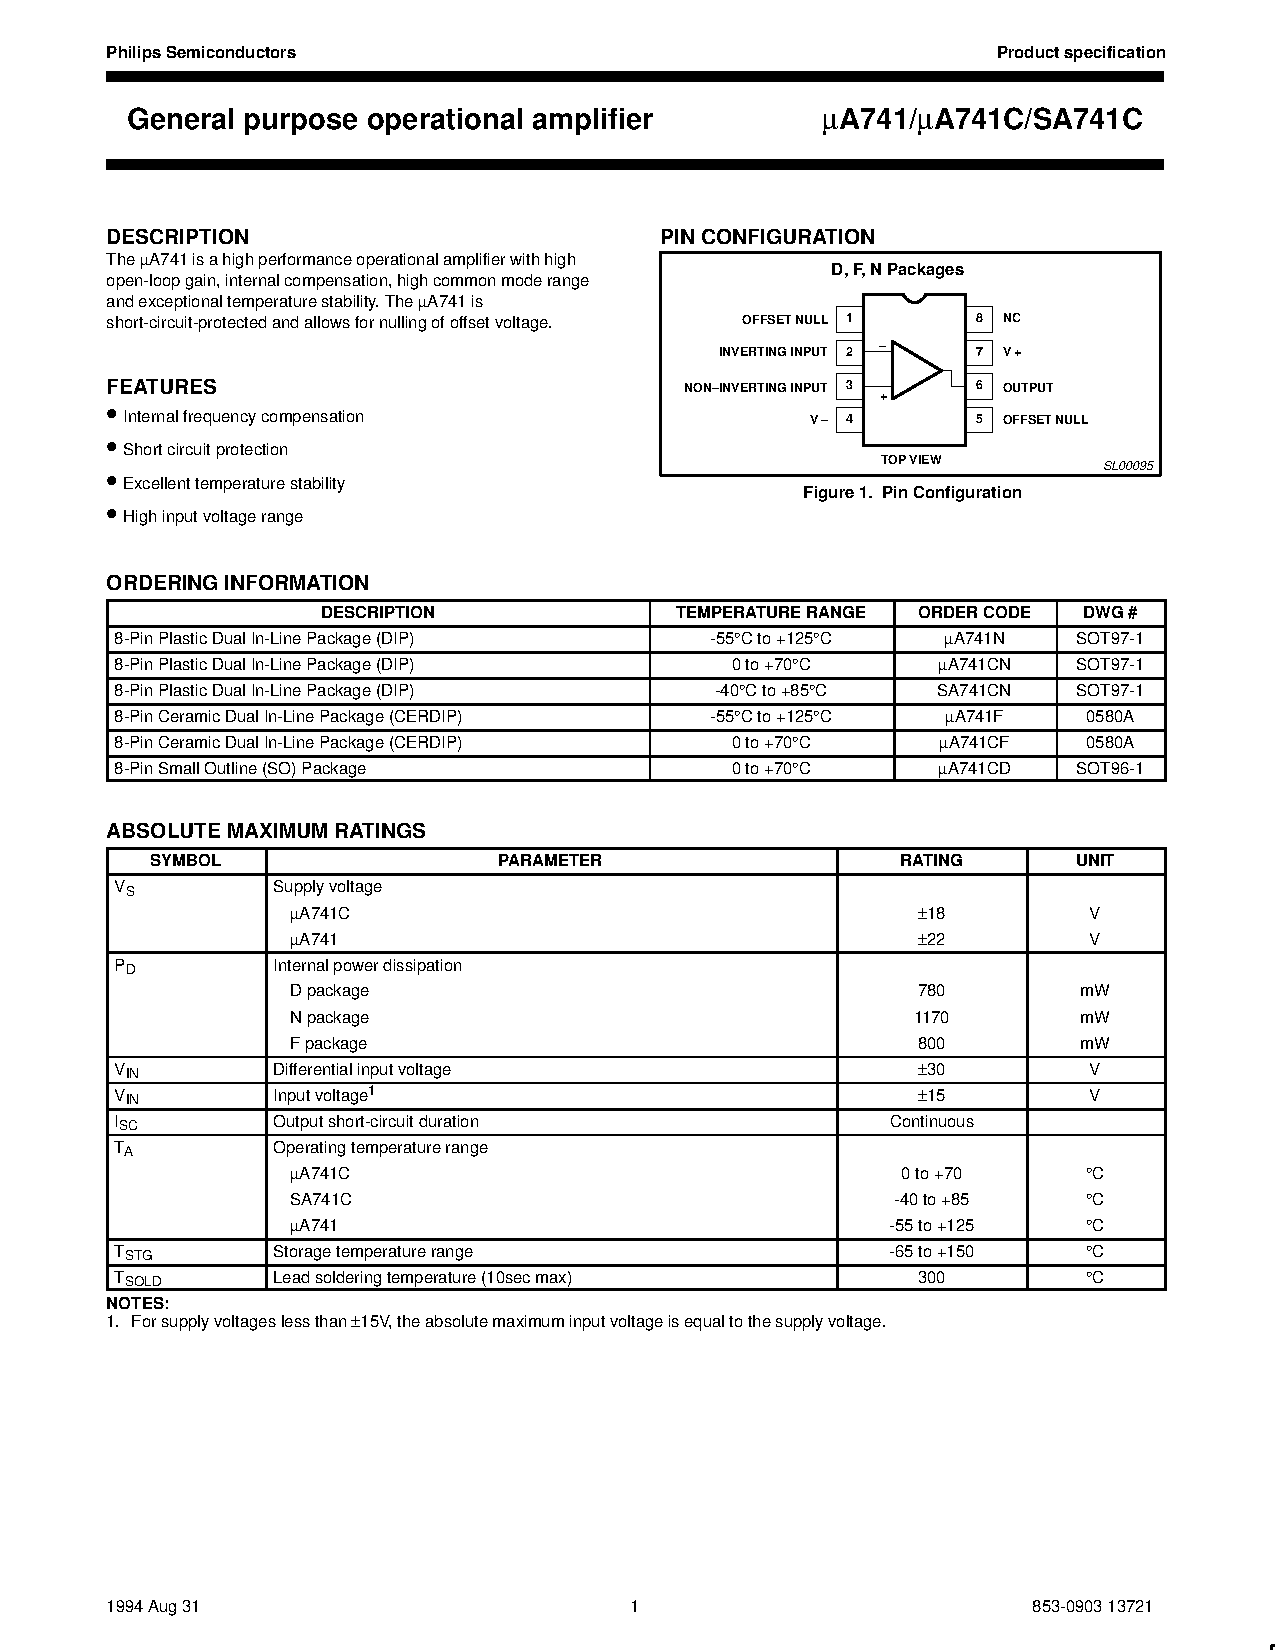
\includepdf[pages={1-6}, nup=1x2, landscape=true]{SecKz_ModKz_Pic_BB.pdf} 
%---------- END  I N C L U D E       P D F
%
%****************************************************************************************************
%============================= E N D   S U B D O C U M E N T  ==========================
%****************************************************************************************************
%
% Verzeichnisse (to be commented out for compilation of main file):
%Im Addendum ist der sogenannte Anhang dargestellt. Beim Verfassen der Dokumentation ist dieser Teil vielleicht noch
%nicht notwendig.
%% Zusammenfassung und Resumee der Diplomarbeit:
\section{Zusammenfassung}

Hier steht die Zusammenfassung und das Resumee der Diplomarbeit!
\newpage

% Anhang zur Diplomarbeit:
\section{Anhang}

Hier stehen zusätzliche Informationen zur Diplomarbeit!
Zum Beispiel können hier Listings oder Teile des Programmes abgebildet sein:

\begin{lstlisting}
// create new document
string path = @"C:\Data\sample.xlsx";
// add title row 
List<string> titleRow = new List<string>();
titleRow.Add("This is the 1st cell");
titleRow.Add("This is the 2nd cell");
openXmlExcel.addTitleRow(titleRow);
// add scatter chart
List<double[]> xValues = new List<double[]>();
List<double[]> yValues = new List<double[]>();
List<string> lineNames = new List<string>();
// first line
xValues.Add(new double[5] { -2, -1, 0, 1, 2 });
yValues.Add(new double[5] { -2, -1, 0, 1, 2 });
lineNames.Add("Line 1");
// second line
xValues.Add(new double[5] { -2, -1, 0, 1, 2 });
yValues.Add(new double[5] { -3, -1, 0, 1, 3 });
lineNames.Add("Line 2");
// save document 
openXmlExcel.saveFile();
\end{lstlisting}

\newpage

\section{Verzeichnisse}
% Bildverzeichnis:
\listoffigures 
%
% Abkürzungsverzeichnis:
%Abkürzungsverzeichnis: Alle Abkürzungen, die bekannt sind finden sich in diesem Verzeichnis.
%Nur diejenigen, die im Dokument auch verwendet werden kommen in die Liste der Compilierung 
%
%der Name der Überschrift kann frei gewählt werden (in diesem Fall: Abkürzungen):
%
%\section*{Acronymverzeichnis}					%Alternative Überschrift für das Verzeichnis
\section*{Abkürzungen}
%
%usage im Dokument: \acs{DA}
%usage im Dokument: \acs{Kurzzeichen}
\begin{acronym}[längstesAcronym]
\setlength{\itemsep}{-0.3 \parsep}
%
% Einträge für Abkürzungen:
%usage im Verzeichnis: \acro{Kurzzeichen}[Inhalt der im Text steht]{Text der als Erklärung im Glossar steht!}
%
\acro{DA}[Diplomarbeit]{Text für die Erklärung der Diplomarbeit}
\acro{ESD}[ESD]{Electrostatic Discharge}
\acro{EMC}[EMC]{Electromagnetic Compatibility}
%
%
% weitere Einträge ...
%
\end{acronym}

%
% Literaturverzeichnis:
%Literaturverzeichnis: Alle Zitate und Veröffentlichungen, die bekannt sind finden sich in diesem Verzeichnis.
%Nur diejenigen, die im Dokument auch verwendet werden kommen in die Liste der Compilierung 
%
%usage im Dokument: \cite{Kurzzeichen}   hier wird im Dokument nur der Text in eckiger Klammer abgebildet
%usage im Dokument: \cite[S~105]{11_Killinger} hier wird auch eine Seitenanzahl dazugestellt
\begin{thebibliography}{22}
%
% Einträge für Literaturverzeichnis:
%usage im Verzeichnis: \bibitem[Werk, Jahrgang oder Auflage]{Kurzzeichen}{Text der als Erklärung im Glossar steht!}
%
   \bibitem[Killinger, 1998]{11_Killinger} Sprache heute : Schriftverkehr; Deutsch für berufsbildende Schulen,\newline 
Seit der Einführung der Bildungsstandards steht der Erwerb fachlicher und sozialer Kompetenzen für Alltag und Beruf im Fokus des Unterrichts.\newline
Autoren: Walter Pirnath, Robert Killinger, Josef Neumüller, 1998
%
\bibitem[vgl. Mustermann, 2020]{12_MM} Skriptum: Test im Zuammenhang mit  ...\newline 
Autoren: Max Mustermann, 2020
%
\bibitem[Werk 1, Jahrgang oder Auflage 1]{BlindzitatKurzzeichen_1}{Text der als Erklärung im Literaturverzeichnis steht!}
%
% weitere Einträge ...
%
\end{thebibliography}
				%ACHTUNG: für die Gesamtcompilierung auskommentieren!!
%Wenn das Addendum auskommentiert ist, dann werden die Zitate im Dokument auch nicht richtig dargestellt.
%Nichts desto Trotz gibt es den Eintrag im Main Dokument auch.
\end{document}


 % Dieses Dokument beinhaltet einen Teil der Gesamtarbeit
\newpage

%
%****************************************************************************************************
%========================= B E G I N   D O C U M E N T   C L O S I N G =======================
%****************************************************************************************************
%
% Anhang der DA 
% Zusammenfassung und Resumee der Diplomarbeit:
\section{Zusammenfassung}

Hier steht die Zusammenfassung und das Resumee der Diplomarbeit!
\newpage

% Anhang zur Diplomarbeit:
\section{Anhang}

Hier stehen zusätzliche Informationen zur Diplomarbeit!
Zum Beispiel können hier Listings oder Teile des Programmes abgebildet sein:

\begin{lstlisting}
// create new document
string path = @"C:\Data\sample.xlsx";
// add title row 
List<string> titleRow = new List<string>();
titleRow.Add("This is the 1st cell");
titleRow.Add("This is the 2nd cell");
openXmlExcel.addTitleRow(titleRow);
// add scatter chart
List<double[]> xValues = new List<double[]>();
List<double[]> yValues = new List<double[]>();
List<string> lineNames = new List<string>();
// first line
xValues.Add(new double[5] { -2, -1, 0, 1, 2 });
yValues.Add(new double[5] { -2, -1, 0, 1, 2 });
lineNames.Add("Line 1");
// second line
xValues.Add(new double[5] { -2, -1, 0, 1, 2 });
yValues.Add(new double[5] { -3, -1, 0, 1, 3 });
lineNames.Add("Line 2");
// save document 
openXmlExcel.saveFile();
\end{lstlisting}

\newpage

\section{Verzeichnisse}
% Bildverzeichnis:
\listoffigures 
%
% Abkürzungsverzeichnis:
%Abkürzungsverzeichnis: Alle Abkürzungen, die bekannt sind finden sich in diesem Verzeichnis.
%Nur diejenigen, die im Dokument auch verwendet werden kommen in die Liste der Compilierung 
%
%der Name der Überschrift kann frei gewählt werden (in diesem Fall: Abkürzungen):
%
%\section*{Acronymverzeichnis}					%Alternative Überschrift für das Verzeichnis
\section*{Abkürzungen}
%
%usage im Dokument: \acs{DA}
%usage im Dokument: \acs{Kurzzeichen}
\begin{acronym}[längstesAcronym]
\setlength{\itemsep}{-0.3 \parsep}
%
% Einträge für Abkürzungen:
%usage im Verzeichnis: \acro{Kurzzeichen}[Inhalt der im Text steht]{Text der als Erklärung im Glossar steht!}
%
\acro{DA}[Diplomarbeit]{Text für die Erklärung der Diplomarbeit}
\acro{ESD}[ESD]{Electrostatic Discharge}
\acro{EMC}[EMC]{Electromagnetic Compatibility}
%
%
% weitere Einträge ...
%
\end{acronym}

%
% Literaturverzeichnis:
%Literaturverzeichnis: Alle Zitate und Veröffentlichungen, die bekannt sind finden sich in diesem Verzeichnis.
%Nur diejenigen, die im Dokument auch verwendet werden kommen in die Liste der Compilierung 
%
%usage im Dokument: \cite{Kurzzeichen}   hier wird im Dokument nur der Text in eckiger Klammer abgebildet
%usage im Dokument: \cite[S~105]{11_Killinger} hier wird auch eine Seitenanzahl dazugestellt
\begin{thebibliography}{22}
%
% Einträge für Literaturverzeichnis:
%usage im Verzeichnis: \bibitem[Werk, Jahrgang oder Auflage]{Kurzzeichen}{Text der als Erklärung im Glossar steht!}
%
   \bibitem[Killinger, 1998]{11_Killinger} Sprache heute : Schriftverkehr; Deutsch für berufsbildende Schulen,\newline 
Seit der Einführung der Bildungsstandards steht der Erwerb fachlicher und sozialer Kompetenzen für Alltag und Beruf im Fokus des Unterrichts.\newline
Autoren: Walter Pirnath, Robert Killinger, Josef Neumüller, 1998
%
\bibitem[vgl. Mustermann, 2020]{12_MM} Skriptum: Test im Zuammenhang mit  ...\newline 
Autoren: Max Mustermann, 2020
%
\bibitem[Werk 1, Jahrgang oder Auflage 1]{BlindzitatKurzzeichen_1}{Text der als Erklärung im Literaturverzeichnis steht!}
%
% weitere Einträge ...
%
\end{thebibliography}
 % Dieses Dokument beinhaltet Zusammenfassungen, Verzeichnisse und den Anhang
%Wenn das Addendum auskommentiert ist, dann werden die Zitate im Dokument auch nicht richtig dargestellt.
%
%****************************************************************************************************
%=============================== E N D   D O C U M E N T  ============================
%****************************************************************************************************
\end{document}



